\chapter{The basic model}\label{ch:The-Exemplar-Model}

One of the earliest \isi{exemplar} models within linguistics, \citet{Goldinger1996}
(adapting \citealt{hintzman1984minerva}), was designed to capture the
effect of past experience on current \isi{perception}. In this model, new
tokens are experienced and added to memory in the following way. First,
the n-dimensional similarity between a novel (``probe'') token and all
members of a given category is calculated. The overall degree of
similarity will determine whether a given probe is recognized or not.
The similarity matrix is, in turn, used to create an ``echo'' of the
probe: the average of the values of each stored token, along each
dimension, weighted by the similarity of that token to the probe. This echo, rather
than the probe itself, is what is then added to memory. These properties
allow the model to simulate the phenomenon whereby listeners often
mistakenly ``remember'' tokens that are particularly ``good'', or prototypical,
members of a category, even when they have never actually experienced
those tokens. Goldinger's model also introduced a \isi{production} component
– a seemingly minimal extension in which a stored echo can be selected
for ``readout''. Goldinger is explicit about assuming that the articulations
needed to produce a given auditory token can be accurately reconstructed
from the acoustics of that token (and thus directly ``read out'' from
the stored \isi{perception} token). This assumption would be implicitly
adopted in most of the work that followed. 

The standard perception-\isi{production} loop model, as well as the application
to sound change \emph{per se}, appears to have originated with \citet{Pierrehumbert2000}.
Production in this model starts with random selection from a store
of perceived tokens. Each \isi{production}, in turn, is then perceived (either
by the original speaker, or by an interlocutor with an identical \isi{exemplar}
space) and then stored. Then the process begins again. In this way,
small perturbations (noise or \isi{articulatory} biases in \isi{production}; perceptual
biases or error in \isi{perception}) accumulate in the \isi{exemplar} cloud, leading
to gradual shifts in the category as a whole. The perception-\isi{production}
loop that will form the basis for the models discussed in this book
is schematized in \figref{fig:Feedback Loop}.

\begin{figure}[H]

\begin{centering}
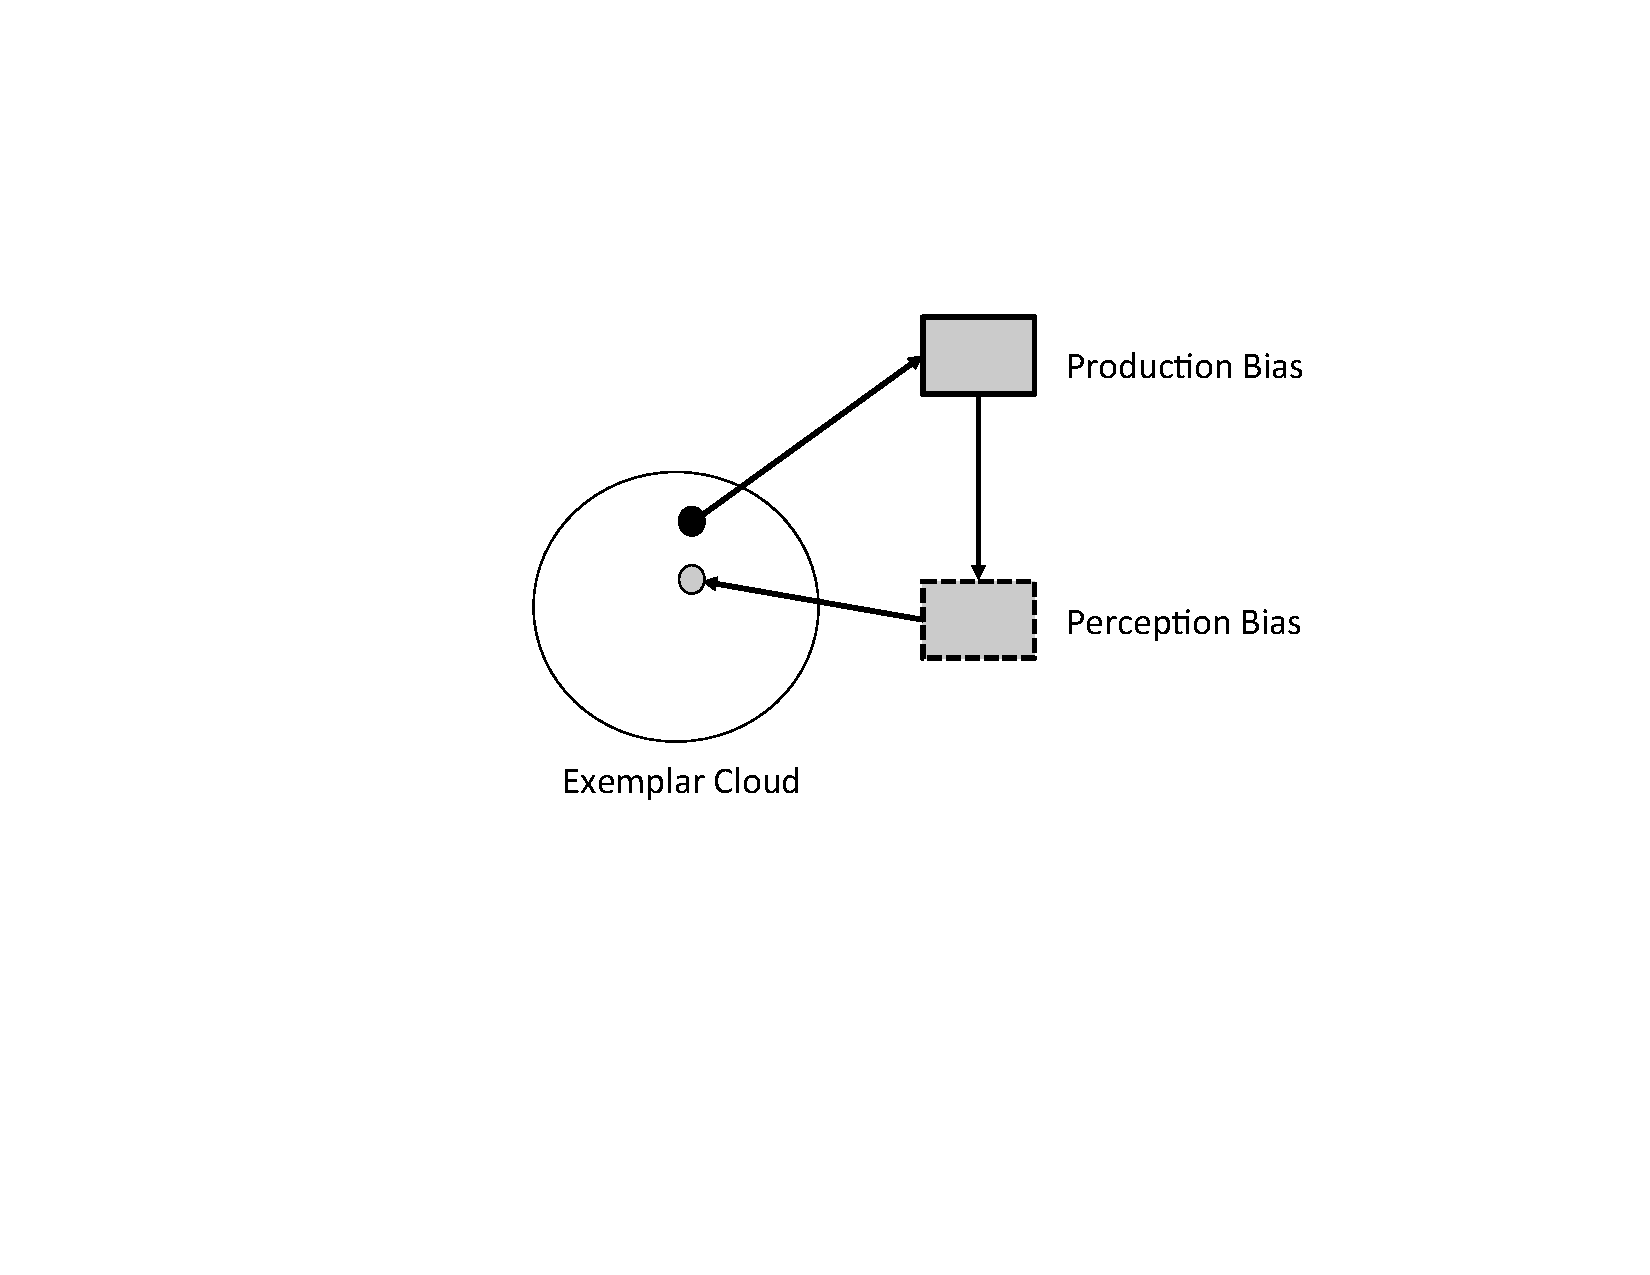
\includegraphics[scale=0.5]{figures/P-PLoop.pdf}\caption{\label{fig:Feedback Loop}Perception-Production Feedback Loop}
\par\end{centering}
\end{figure}

The basic \isi{exemplar} model includes three additional mechanisms that
are necessary for generating useful results. The first of these is
what is typically conceptualized as an error term. This allows for
variation to persist, and provides the necessary stochastic element
needed for achieving multiple outcomes. The second is \isi{entrenchment},
which prevents categories from losing cohesion and dispersing along
the dimensions of variation. The third mechanism is \isi{memory decay},
privileging more recent perceptions in memory, and preventing the
category from simply getting larger and larger. \figref{fig:Baseline-Model-Specification}
is a schematic of the basic algorithm for the models that will be
implemented and run below. Mathematical details will be provided in
the following section and the Appendices. 

\begin{figure}
\noindent\fbox{\begin{minipage}[t]{1\columnwidth - 2\fboxsep - 2\fboxrule}%
Baseline Perception-Production Model (one dimensional)
\begin{enumerate}[label=(\alph*)]
\item Initialize cloud
\begin{itemize}
\item assign values to a cloud of \emph{n} tokens (randomly generated from
a normal distribution of mean $\mu$ and variance $\sigma^{2}$)
\item assign each token an age (a time at which it was produced)
\end{itemize}
\item \label{enu:step 2}Randomly select a token for \isi{production}
\begin{itemize}
\item add the \isi{production} \isi{bias}, moving the token a small amount in the biasing
direction
\item add the error term, moving the token a small amount in either direction
\item add \isi{entrenchment}, moving the token a small amount closer to the category
mean 
\end{itemize}
\item Store
\begin{itemize}
\item add the new token value to the cloud
\item remove one of the oldest tokens from the cloud
\end{itemize}
\item Return to Step \ref{enu:step 2}
\end{enumerate}
\end{minipage}}
\caption{\label{fig:Baseline-Model-Specification}Baseline Model Specification}
\end{figure}


\section{Entrenchment}

Category consolidation, or variance reduction, has been motivated
as an effect of practice, or motor tuning (e.g. \citealp{saltzman1989dynamical}).
Implementationally, it is necessary to prevent the category expansion
in both directions that would result from consistent \isi{production} error,
and the additional expansion that would occur in the biasing direction.
The general equation for \isi{entrenchment} that will be used in this paper
is the following (based on \citealt{Pierrehumbert2000}):
\begin{equation}
E(x_{i})=\epsilon(\bar{x}-x_{i})\label{eq:Entrenchment}
\end{equation}
where $\epsilon$ is a constant between 0 and 1, $x_{i}$ is the current
location of token \emph{i} along some dimension \emph{x}, and $\overline{x}$
is the current category mean along that dimension. Figure \ref{fig:First Model param}
illustrates the evolution of a single \isi{exemplar} cloud generated from
the model outlined in \figref{fig:Baseline-Model-Specification}. In
each sub-figure the different colors indicate the same distribution
at initialization (white), and after a certain fixed number of model
iterations (black). Unless otherwise stated, all models are assumed
to be one-dimensional along \emph{x}. Individual tokens are given
as counts over successively binned \emph{x} values. 

\figref{fig:Basic-Iterative-Model} shows how the distribution as
a whole shifts in the direction of the \isi{production} \isi{bias} over time (measured
in iterations of the perception-\isi{production} loop). \figref{fig:NoEntrenchment}
shows the result of running the same model, minus the \isi{entrenchment}
term, over the same number of iterations. The biasing shift still
occurs, but with increasing variance along the biased dimension. See
Appendix \ref{chap:Appendix A} for the specific parameter values
used in these, and the following, simulations. 

\section{Memory decay}

Without \isi{memory decay}, categories can only spread without shifting.
The older the tokens, the more times, on average, they will have been
chosen as \isi{production} targets, reinforcing the initial conditions of
the cloud. Figure \ref{fig:No-memory-decay:} is an illustration of
this effect for the same model and starting conditions as the previous
two simulations, but with the \isi{memory decay} term removed. No tokens were
discarded. The skew in the direction of the \isi{production} \isi{bias} (implemented
as an incrementally decreasing function) can be seen in the left tail
of the distribution, but older tokens keep the category anchored at
the right. There are a number of ways in which a \isi{memory decay} term
can be implemented. In these and the following models, the total
number of tokens is kept constant by removing one of the oldest tokens
each time a new token is added.\footnote{There are other ways to keep the number of category members constant.
The token furthest from the mean could be discarded on each iteration,
for example. This would act to increase the \isi{entrenchment} effect, further
reducing variation. However, the purpose here is not only to keep
the number of tokens constant, but to allow a domino effect to develop
by increasing the probability that a token will be chosen again with
each biasing iteration. }

\begin{figure}[H]
    \begin{subfigure}[t]{.3\textwidth}
        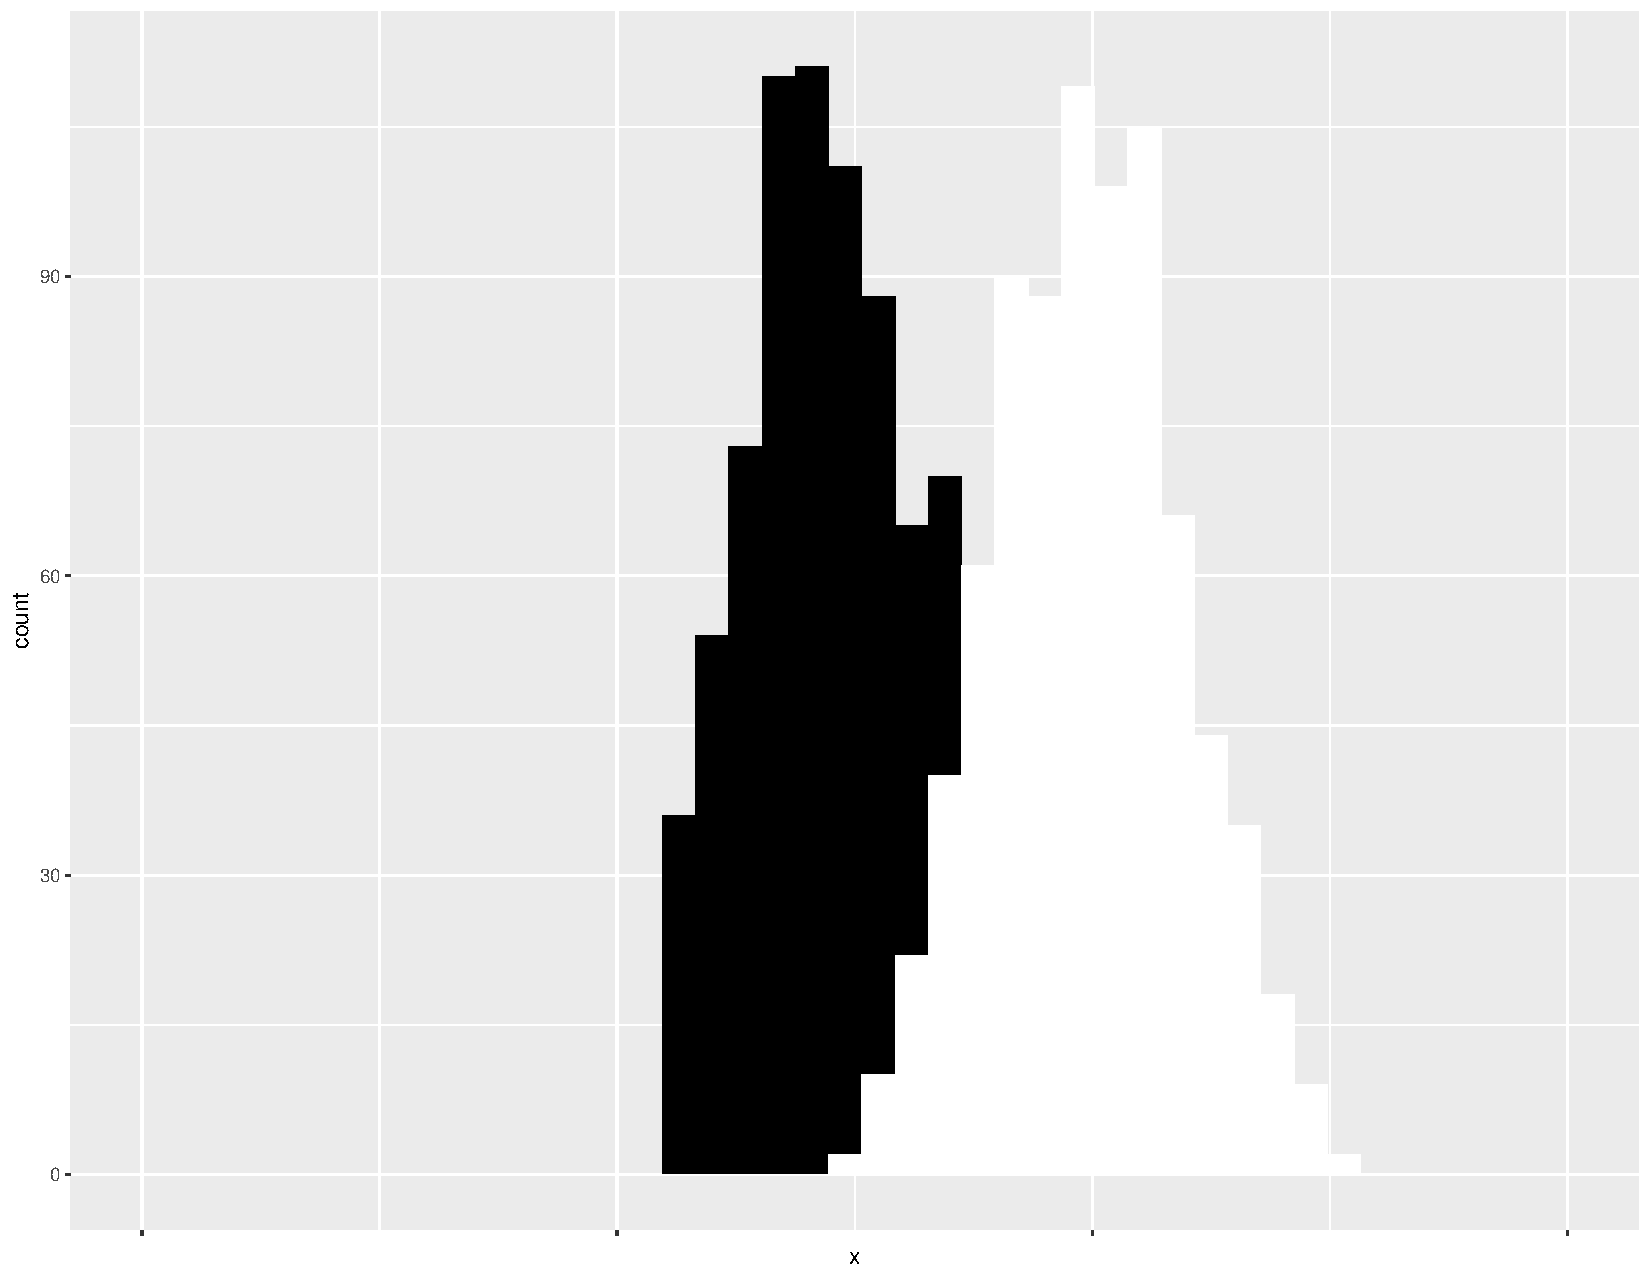
\includegraphics[width=\linewidth]{figures/8000iterwithentrenchment.pdf}
        \caption{\label{fig:Basic-Iterative-Model}All Forces}
    \end{subfigure}\hfill
    \begin{subfigure}[t]{.3\textwidth}
        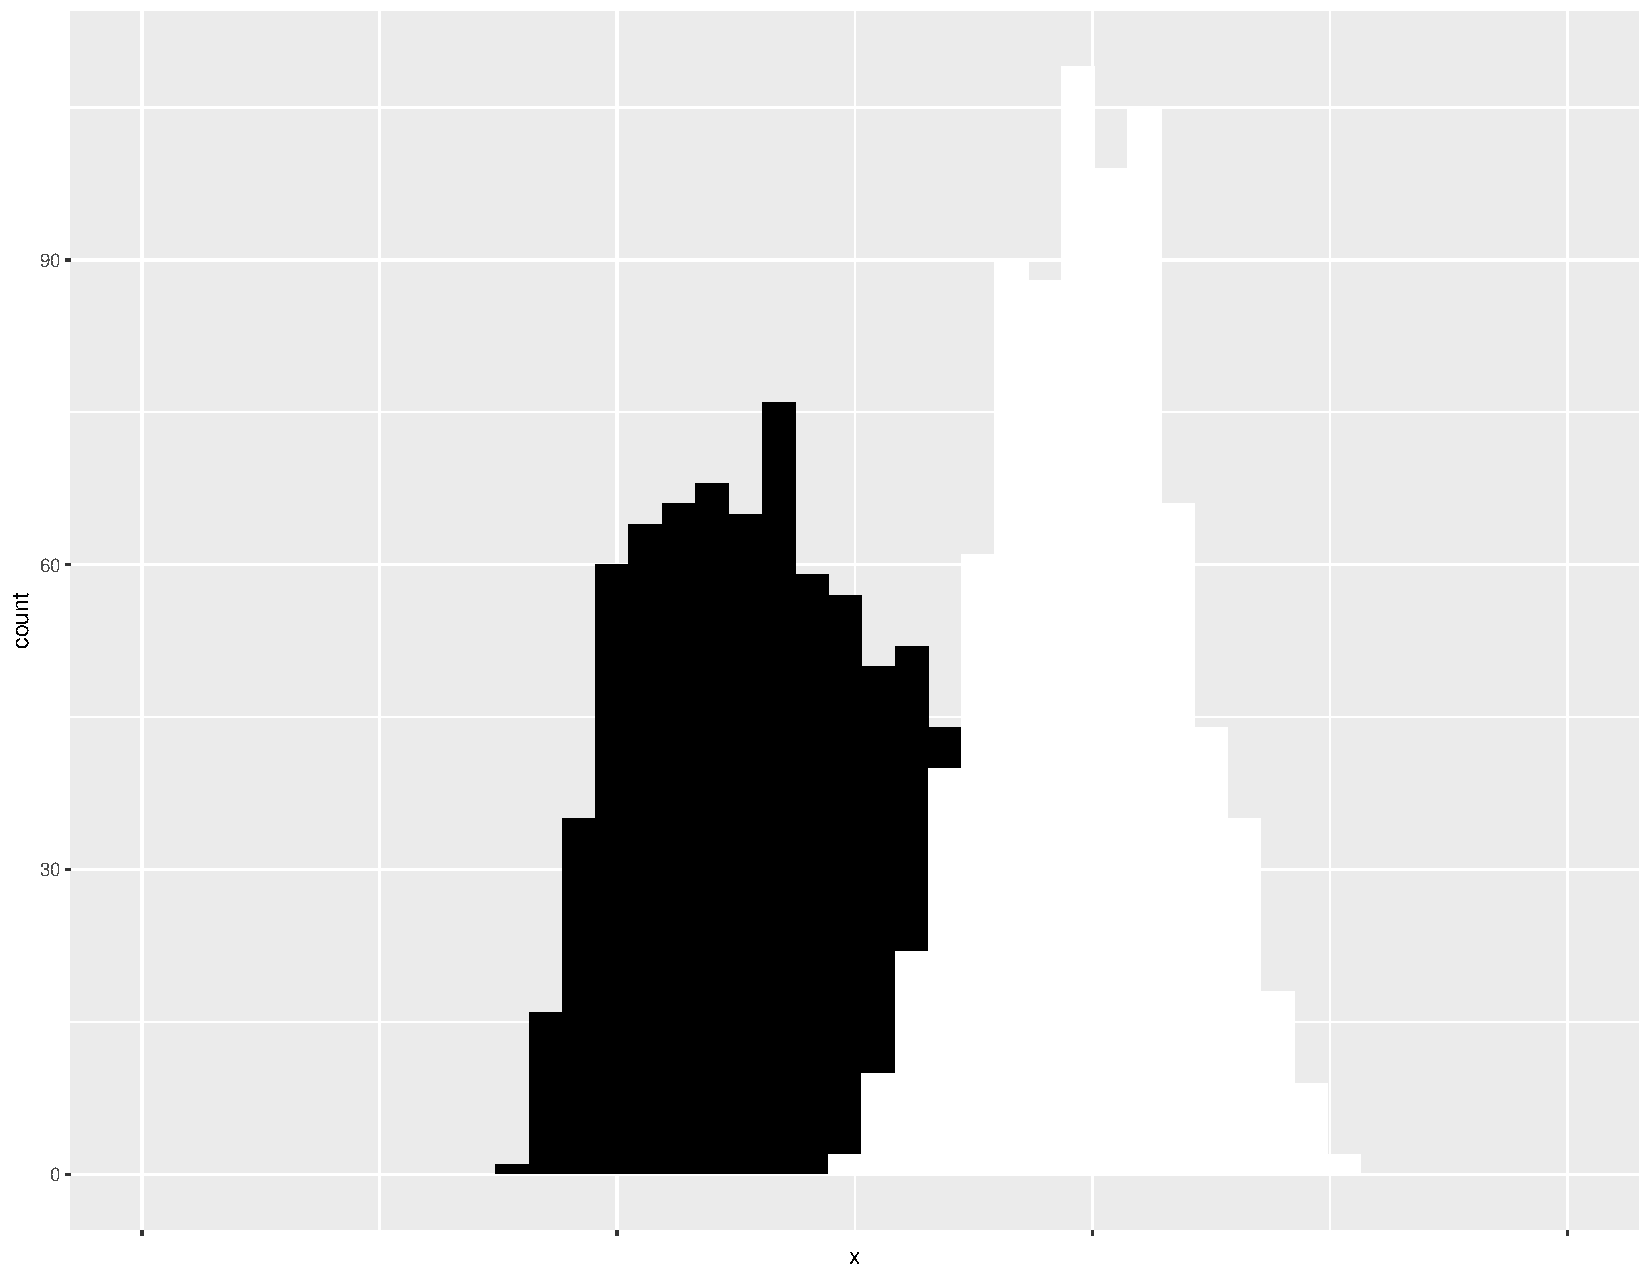
\includegraphics[width=\linewidth]{figures/8000iternoentrenchment.pdf}
        \caption{\label{fig:NoEntrenchment}Without Entrenchment}
    \end{subfigure}\hfill
    \begin{subfigure}[t]{.3\textwidth}
        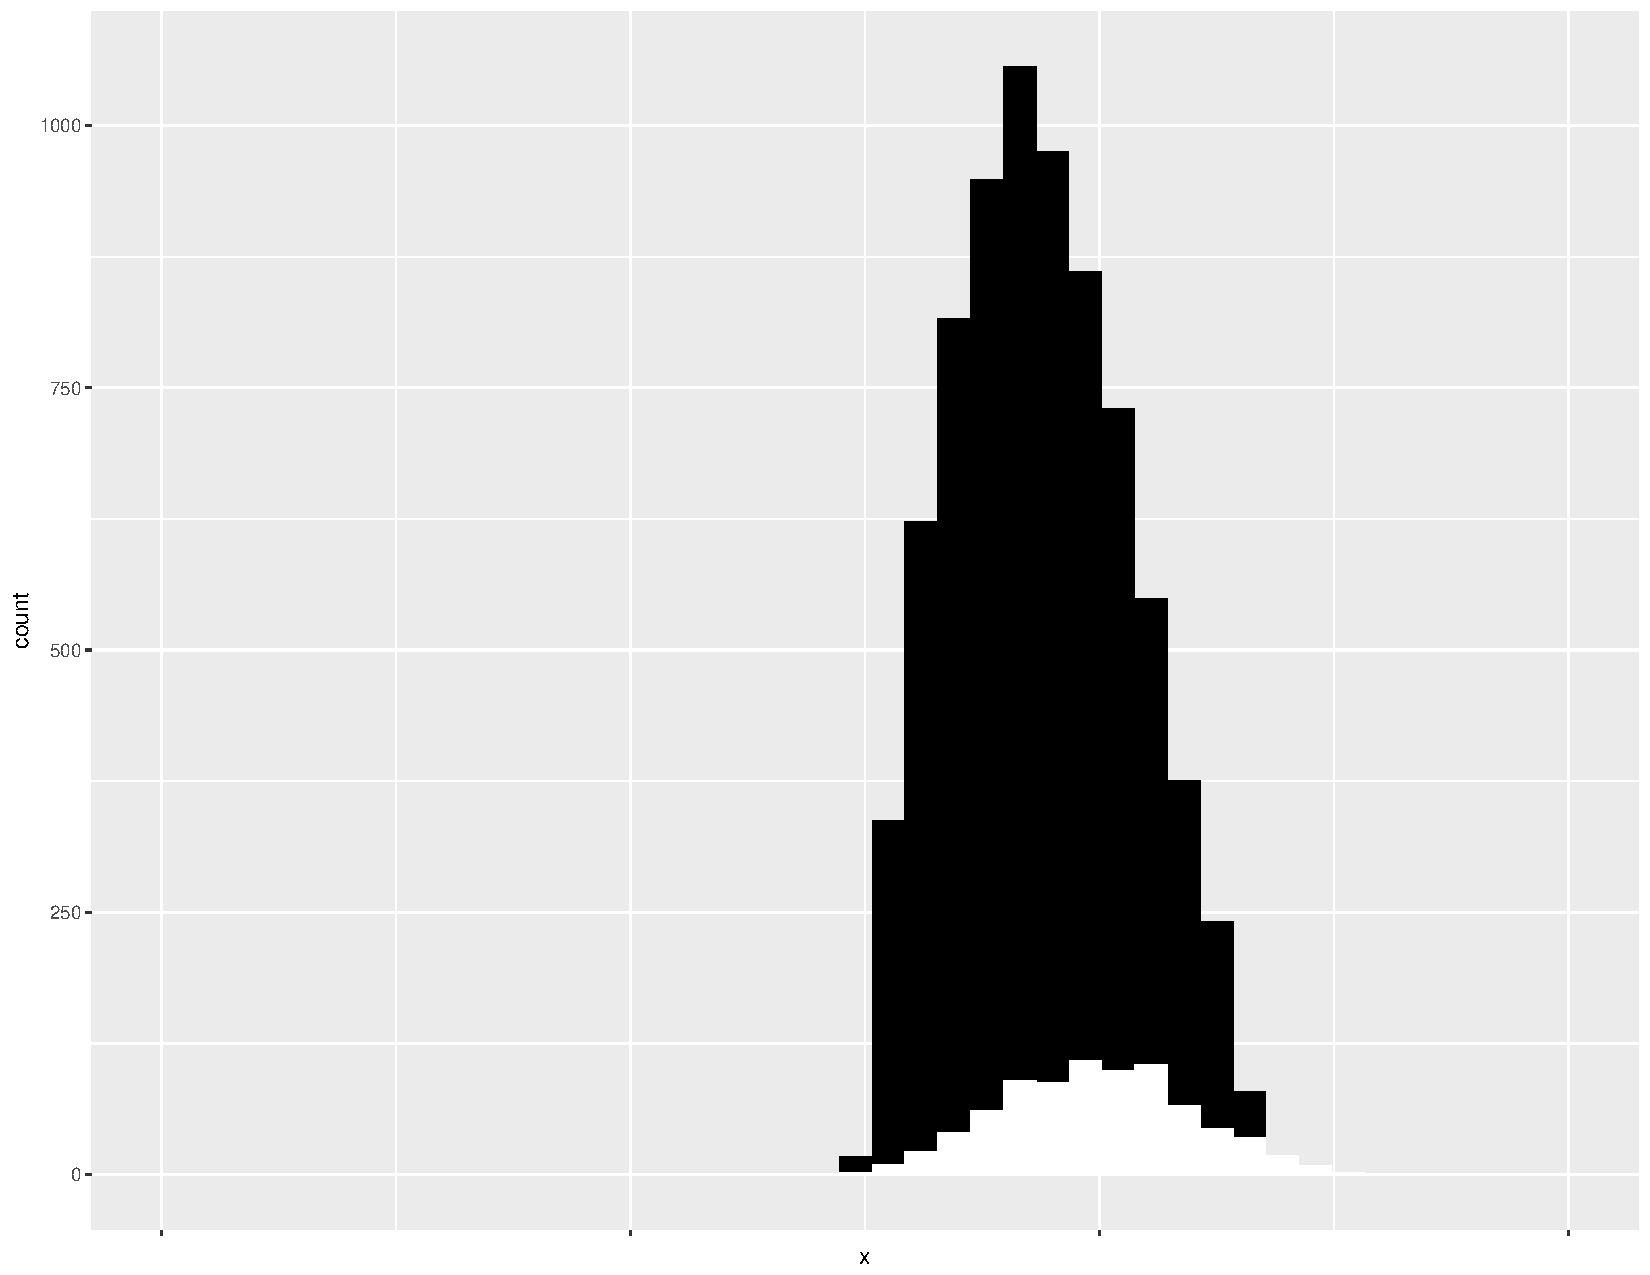
\includegraphics[width=\linewidth]{figures/8000iternomemory.pdf}
        \caption{\label{fig:No-memory-decay:}Without Memory Decay}
    \end{subfigure}
% % % \subfigure[\label{fig:Basic-Iterative-Model}All Forces]{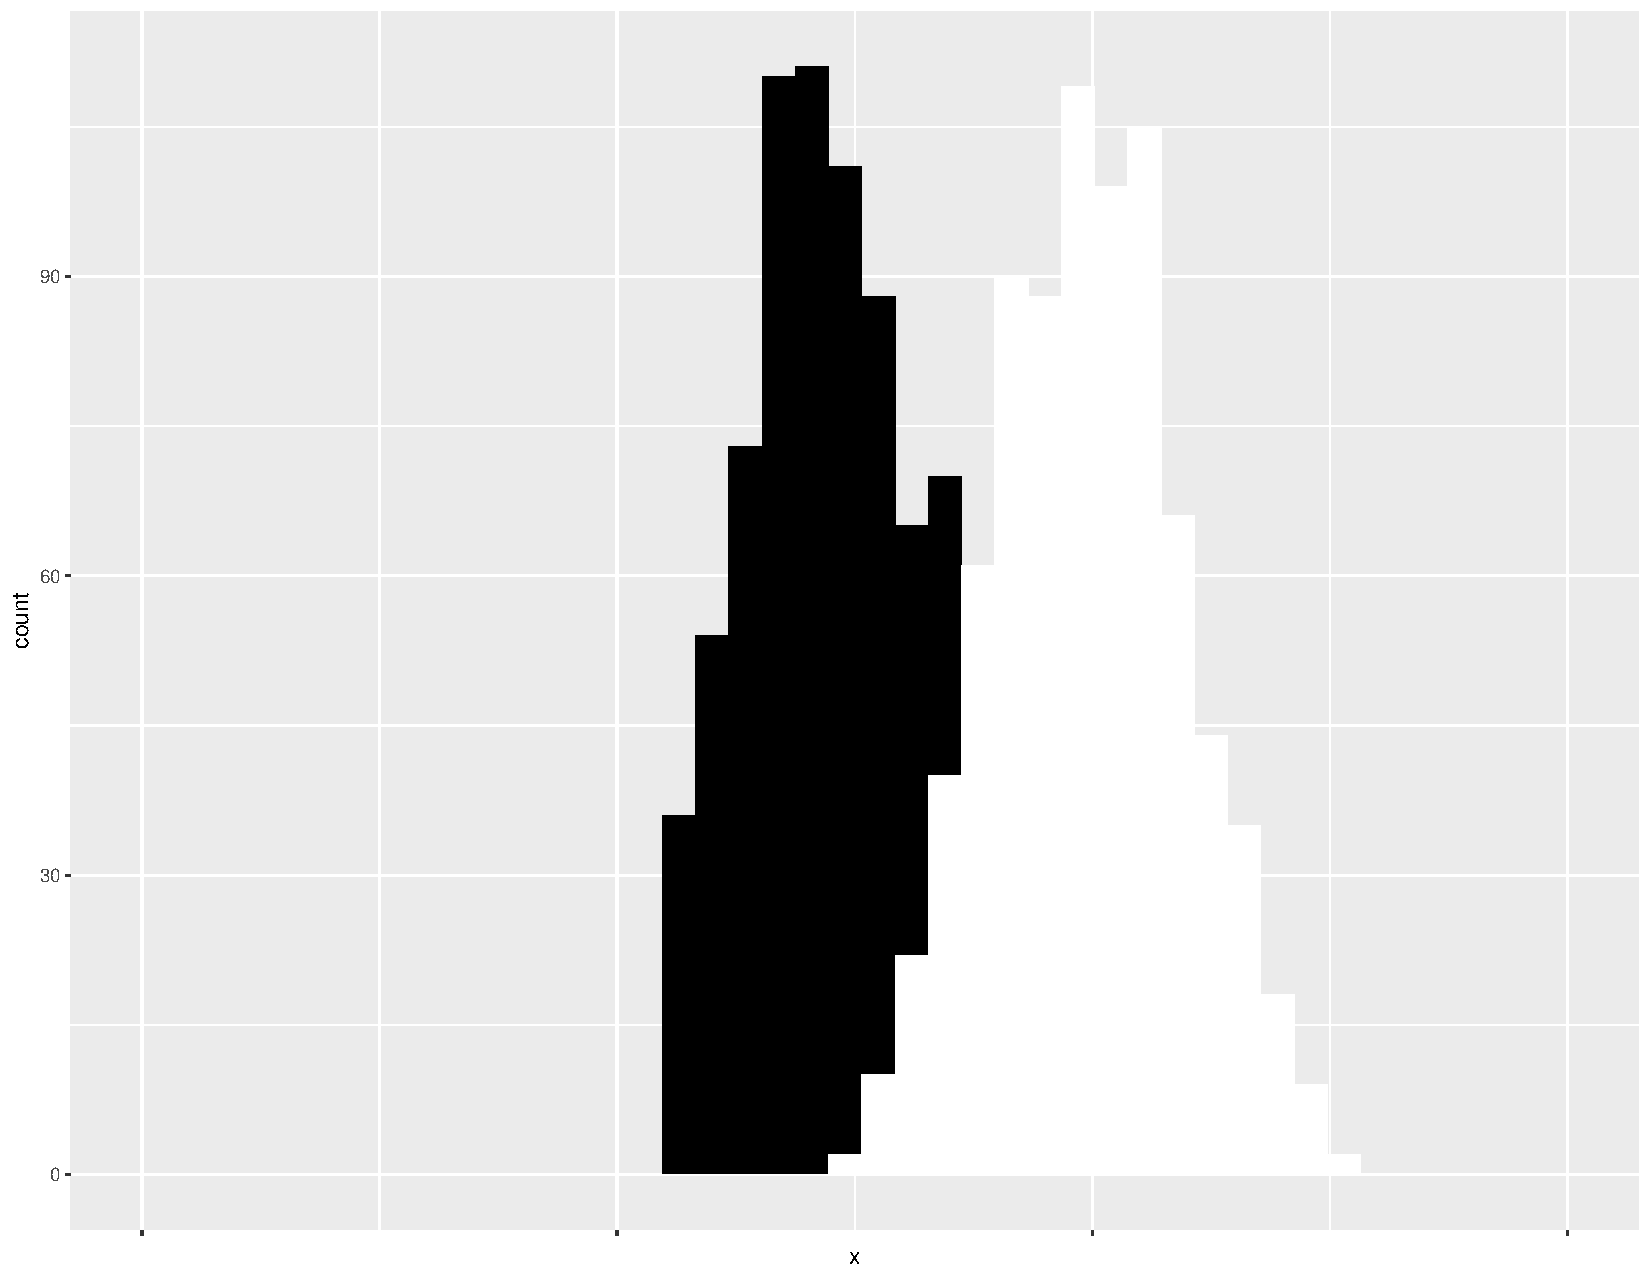
\includegraphics[width=0.25\textwidth]{figures/8000iterwithentrenchment.pdf}}\qquad
% % % \subfigure[\label{fig:NoEntrenchment}Without Entrenchment]{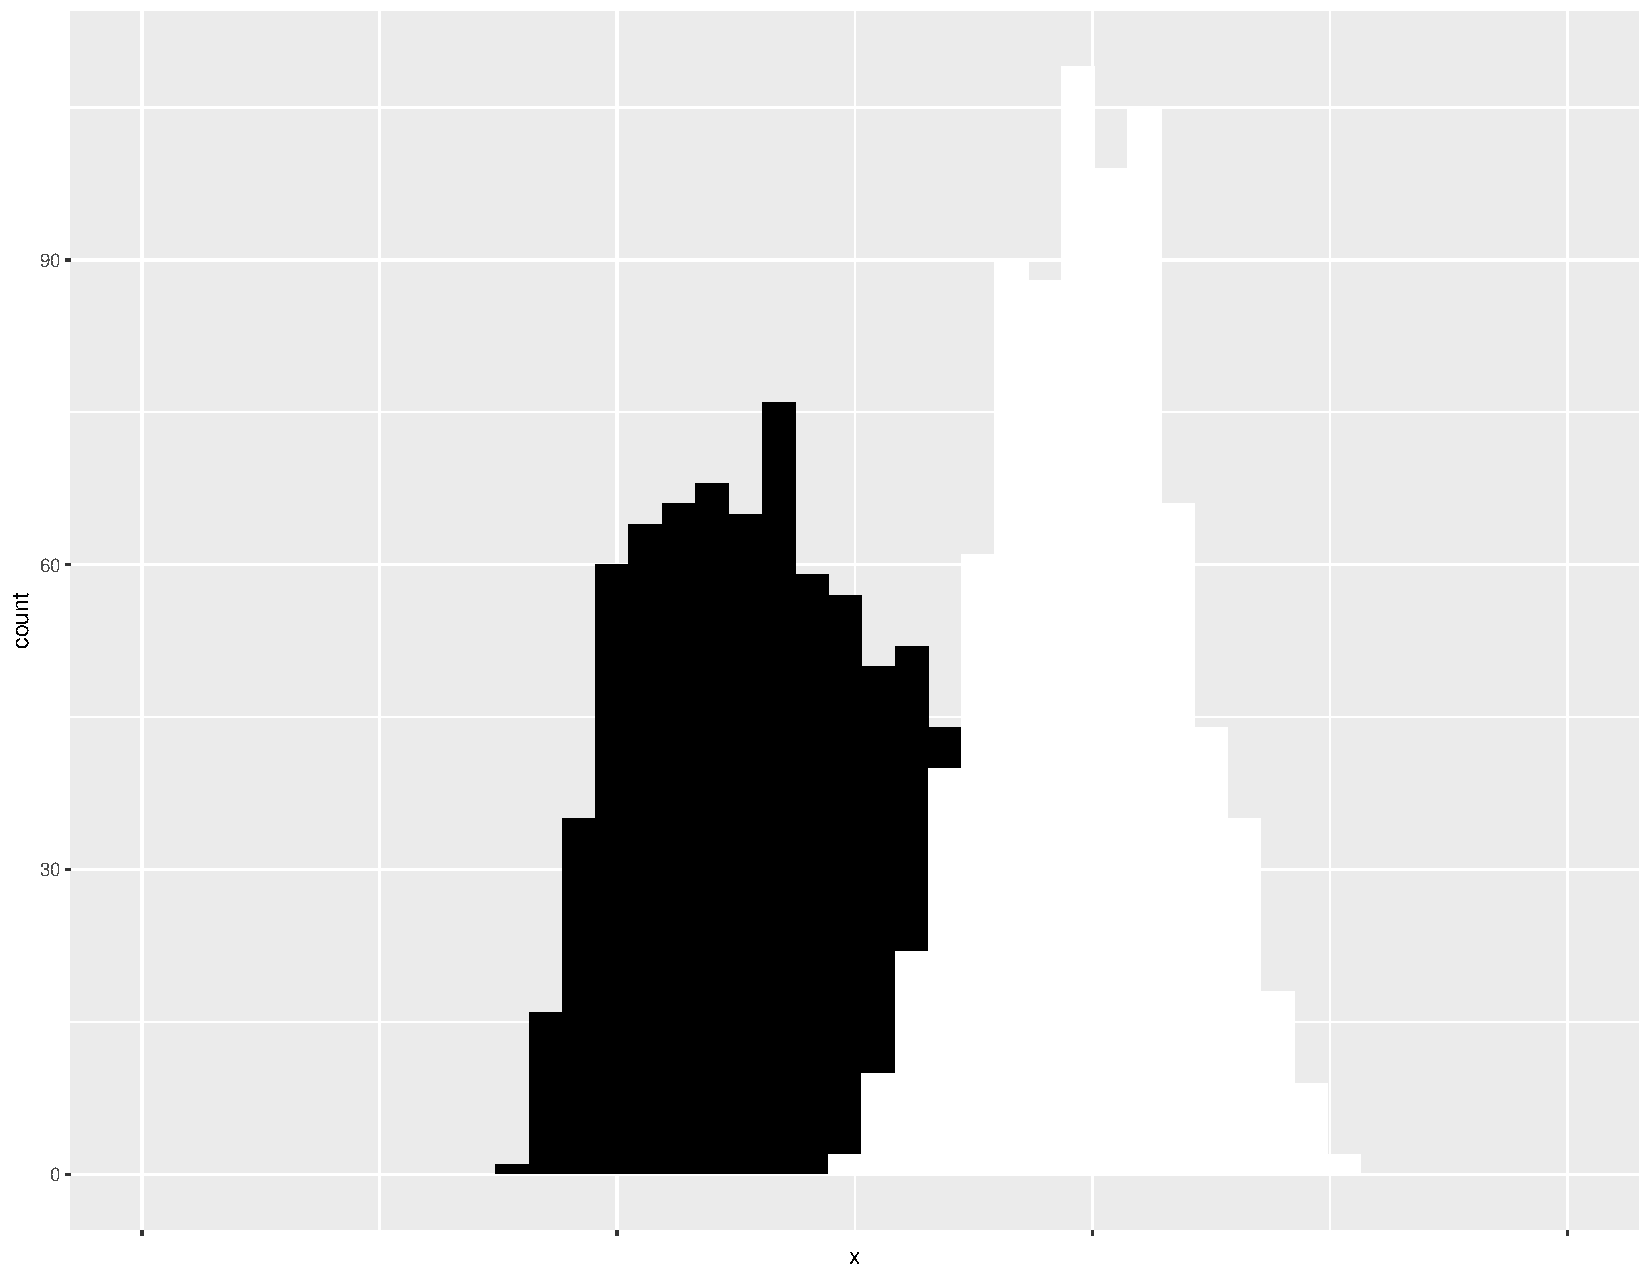
\includegraphics[width=0.25\textwidth]{figures/8000iternoentrenchment.pdf}}\qquad
% % % \subfigure[\label{fig:No-memory-decay:}Without Memory Decay]{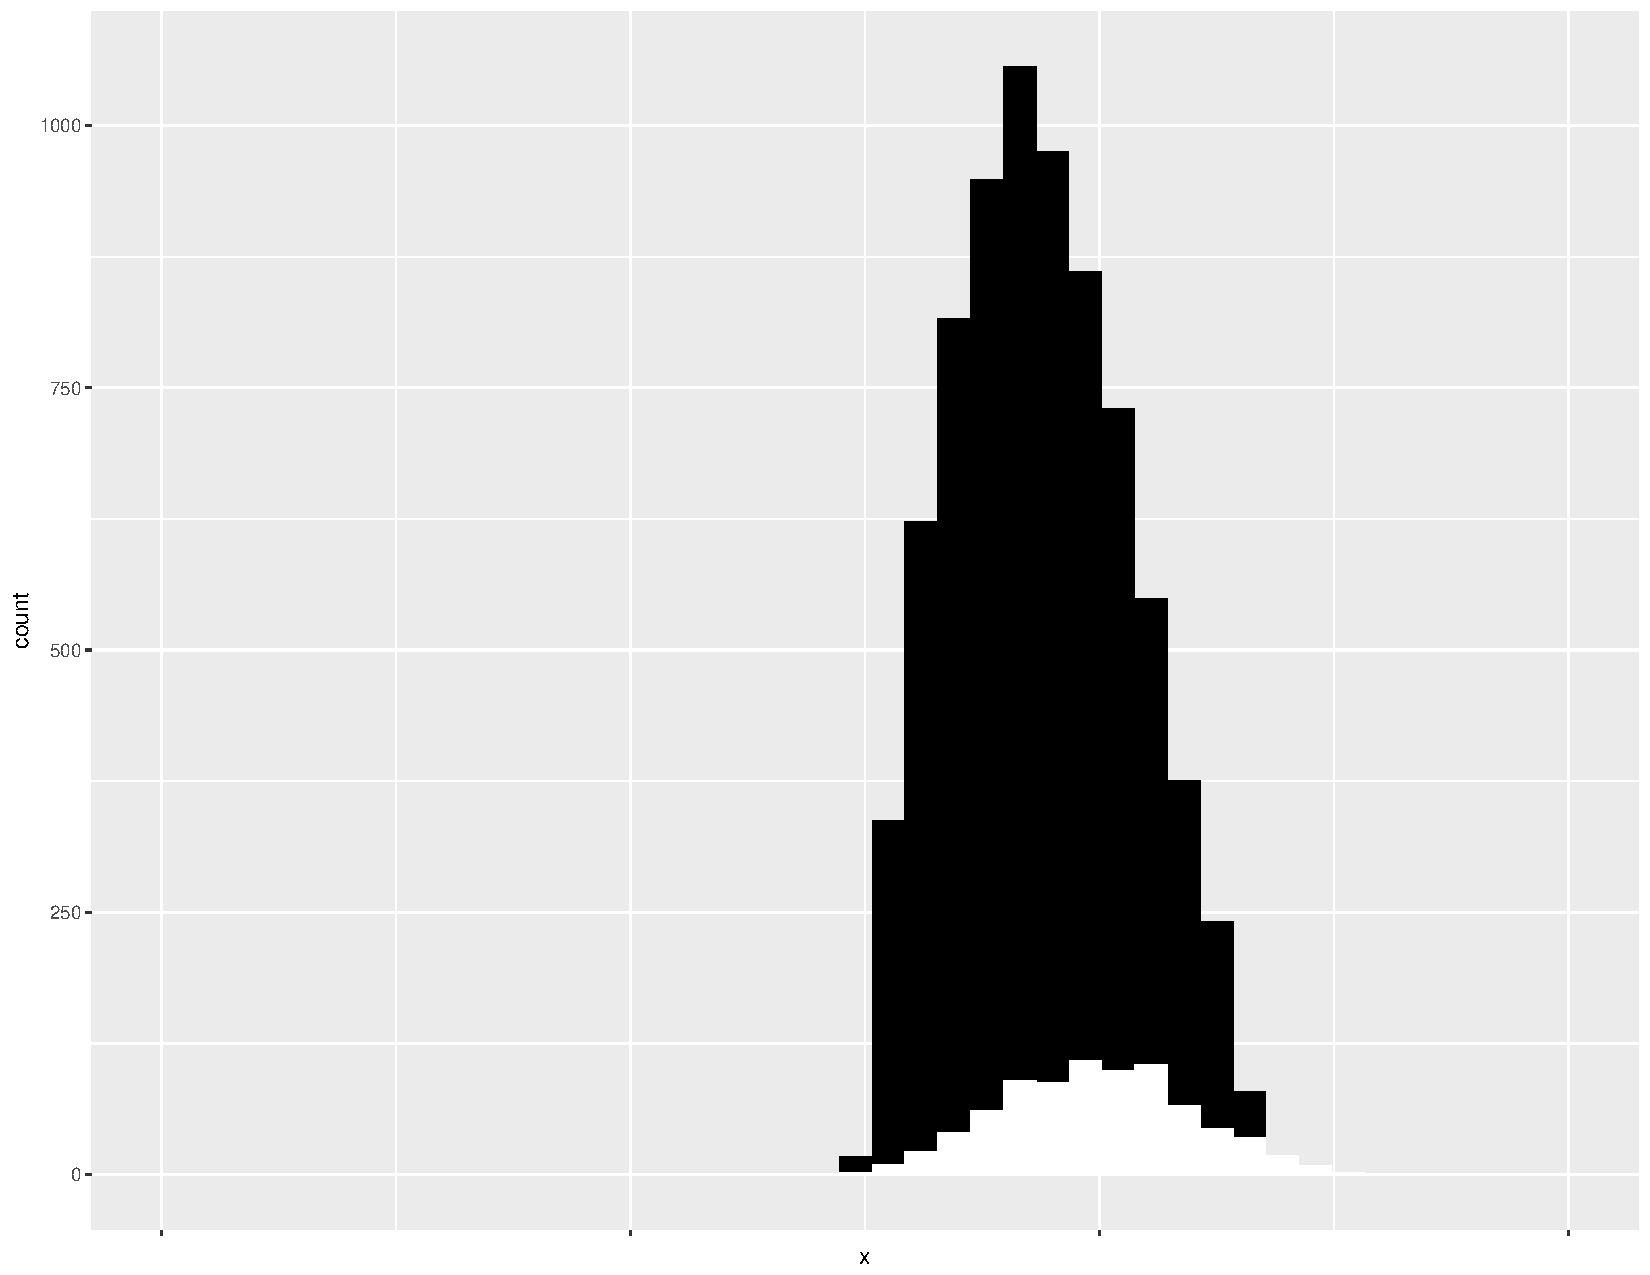
\includegraphics[width=0.25\textwidth]{figures/8000iternomemory.pdf}}
\caption{\label{fig:First Model param}Basic Iterative Model: Starting distribution
(white); Distribution after 8000 iterations (black). Note that y-axis
range in c) is about 10 times larger than in a) and b).}
\end{figure}


\section{\label{sec:Iterativity}The collapse problem}

As illustrated in \figref{fig:Basic-Iterative-Model}, the basic
\isi{exemplar} model with a single unidirectional \isi{bias} can produce cohesive
movement of an entire cloud of exemplars in the direction of the \isi{bias}.
What will be demonstrated in this section is that this shift is unbounded,
leading ultimately to category collapse and merger. This could easily
be inferred from the fact that the basic model contains only one force
that acts in a consistent direction, with nothing to oppose it. However,
it is worthwhile to actually run the simulations for a number of reasons.
Unambiguously establishing the results for general classes of phenomena
will allow us to see immediately what the model predicts for the linguistic
phenomena that map to each of those classes. Running actual simulations
will also force us to consider the question of whether \isi{exemplar} models
are to be evaluated only at convergence, and what the relationship
is between model time and real time, in terms of experiences of instances
of speech. Finally, the specific ways in which the models fail will
be informative regarding the mental representations they are meant to instantiate.

The three classes of phenomena to be modeled in this section are the
following: a context-free process; and two context-dependent processes, 
one gradient, and one categorical. For all of the three basic models,
a \isi{production} \isi{bias}, \emph{B}, will be implemented for a given token
\emph{i}, as a fixed percentage reduction ($\alpha$) in the value
of \emph{$x_{i}$} along dimension \emph{x}. See Eq. (\ref{eq:Production Bias}).\footnote{The \isi{production} \isi{bias} in \citet{Pierrehumbert2000} is a constant that
applies regardless of the current token value. Making the \isi{bias} proportional
results in less reduction for tokens that already have small values, thus
fixing the percentage of reduction, rather than the absolute value,
for all tokens.} 
\begin{equation}
B(x_{i})=-x_{i}\alpha\label{eq:Production Bias}
\end{equation}
After the \isi{production} \isi{bias} applies, the biased token will be added
back to the cloud from which it was originally drawn. It will be useful
to express the value of a given token on any iteration as a function
of the original non-biased token that gave rise to it. For one such
original token, $x_{i}$, we can label its biased daughter as $x_{i(+1)}$,
and calculate its biased value to be $x_{i}(1-\alpha)$
along dimension \emph{x}. If, on some subsequent iteration, this daughter
token $x_{i(+1)}$ is chosen for \isi{production}, it will be subject to
the same biasing force, resulting in the granddaughter, $x_{i(+2)}$,
with value $x_{i(+2)}=x_{i(+1)}(1-\alpha)=x_{i}(1-\alpha)^{2}$.
Proceeding to the general case, we can express the value of any token,
on any given model iteration, as a function of the value of its originator
token ($x_{o}$), and the number of generations, \emph{n}, by which
the current token is removed from that originator. See Eq. (\ref{eq:linear bias}). 
\begin{equation}
x_{o(+n)}=x_{o}\left(1-\alpha\right)^{n}\label{eq:linear bias}
\end{equation}


\subsection{\label{subsec:Model-1:-Context-Free}Model 1: Context-free iterativity}

In Model 1, the \isi{bias} function applies to all tokens. Therefore, the
linear \isi{bias} term in (\ref{eq:linear bias}) will cause the entire
category to shift in the biasing direction over time. The following
simulations compare the behavior of a low-\isi{frequency} category, to a
high-\isi{frequency} category, one whose tokens are produced, and thus experienced,
more often. All simulations begin with the same starting distributions:
a high-\isi{frequency} category with 800 tokens, and a low-\isi{frequency} category
with 200 tokens. Steps were taken to make the distributions of the
two categories as close as possible.\footnote{The high-\isi{frequency} category was generated by randomly sampling 800
tokens from a normal distribution with mean of $50x$ and a standard
deviation of $2x$. The low-\isi{frequency} category was then created by
sampling 200 tokens from the high-\isi{frequency} category: 50 tokens from
each quartile.} See Figure \ref{fig:Frequency Starting Dist}. 

\begin{figure}[H]
\centering{}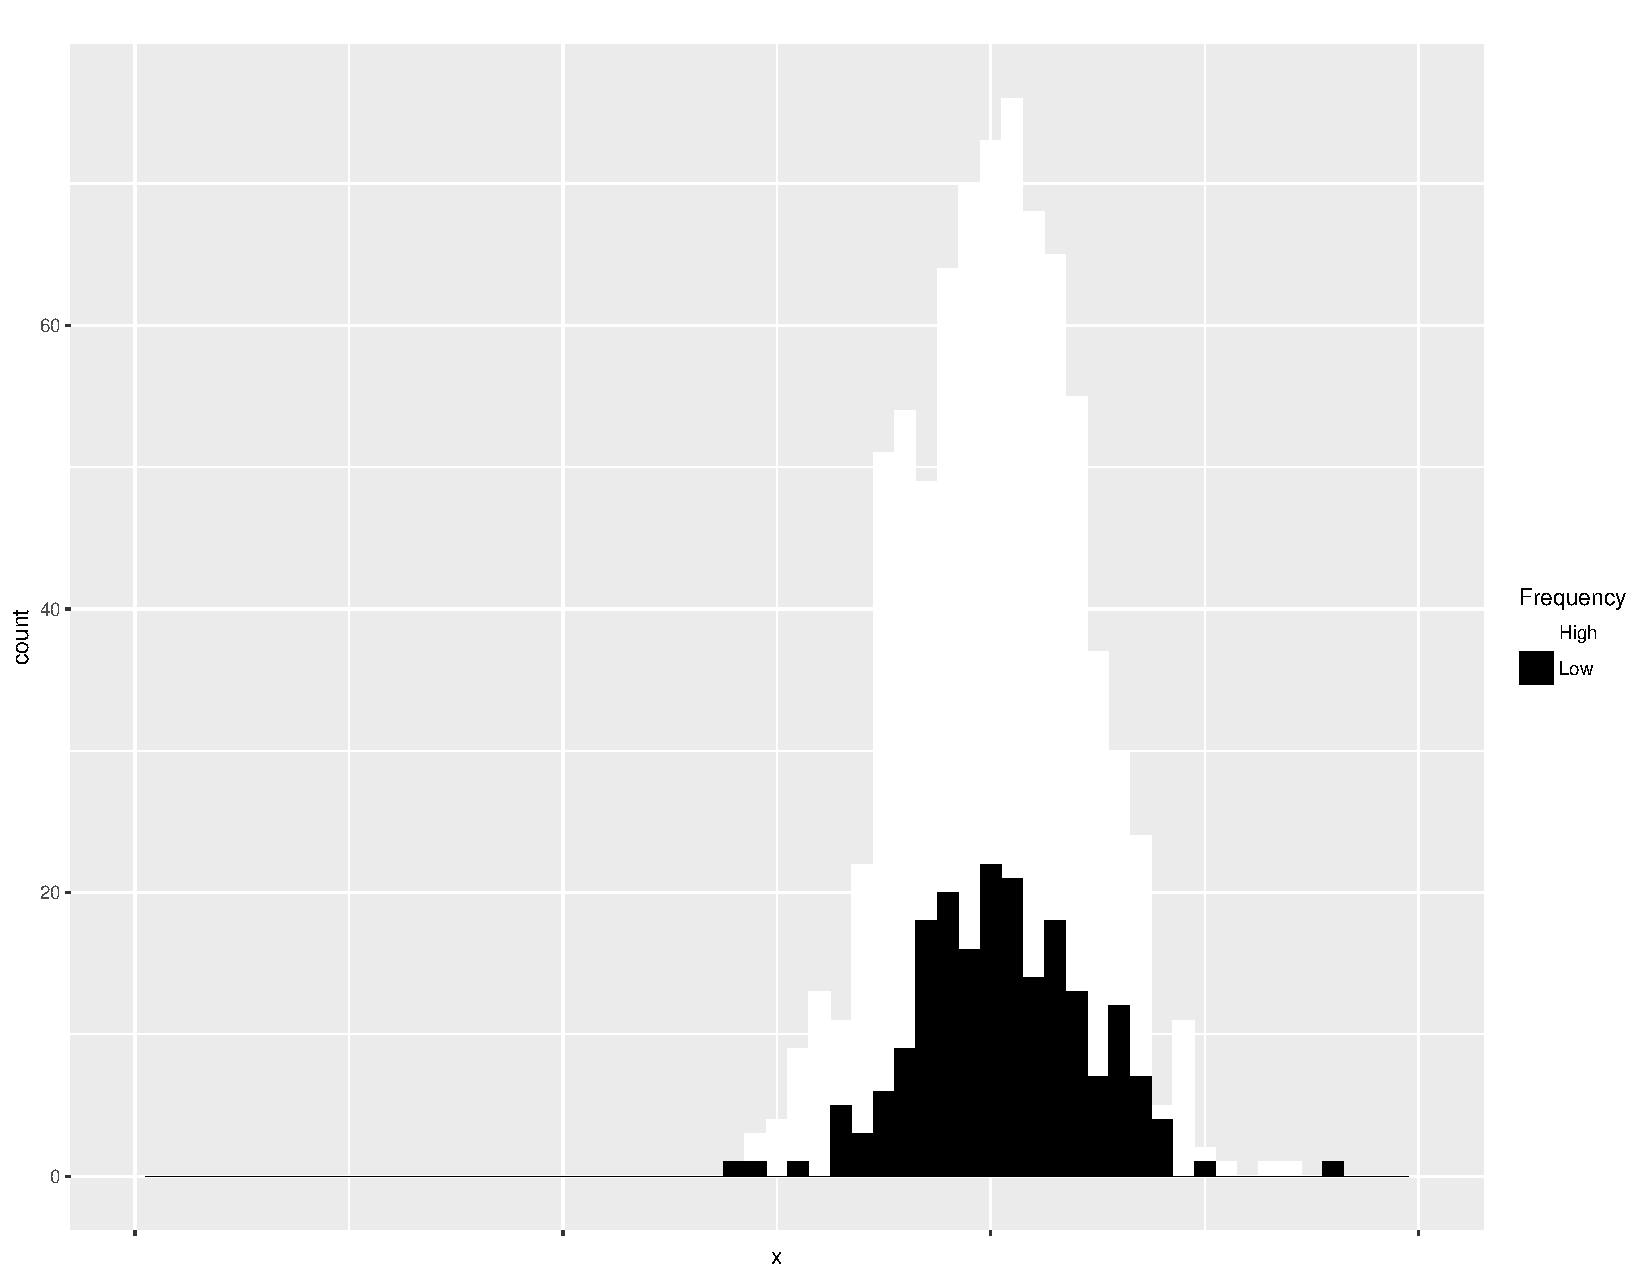
\includegraphics[scale=0.25]{figures/startCon.pdf}\caption{\label{fig:Frequency Starting Dist}Starting Distribution. White bars:
High-frequency category. Black bars: Low-frequency category.}
\end{figure}

Because these models rely on random processes, the outcome is not
guaranteed to be identical each time the model is run. To evaluate
models of this kind, one conducts a number of independent identical
``experiments'' (trials) that consist of running the model with the
same starting conditions, and the same parameters, for the same number
of iterations. Results are then averaged over the set of trials. In
the first set of simulations, 500 model trials were run for 1000 iterations
each. On each model iteration one token was produced, selected stochastically
from among all possible tokens (making it 4 times more likely to be
chosen from the high-\isi{frequency} than the low-\isi{frequency} category). That
token was biased according to Eq. (\ref{eq:Production Bias}) and
then added back to the category from which it originated. 

The mean category value along \emph{x} for each category was calculated
at the end of each of the 500 trials, and converted to a z-score.
A boxplot of the difference between the means of the two categories
on each trial is shown in \figref{fig:HvL}. In 44\% of trials the
difference was negative (low-\isi{frequency} mean larger than high-\isi{frequency}),
and in 56\% it was positive. The mean difference over all 500 trials
was close to zero: 0.031 (or 16\% of the initial distribution standard
deviation). Thus we do not see a consistent difference in the two
categories after an arbitrarily selected number of iterations. Intuitively,
we might have expected the higher-\isi{frequency} category to have moved
further along \emph{x}, and have a lower value, because tokens from
that category are produced more often, and thus multiply-biased.
However, it is also the case that, if \isi{frequency} of occurrence is expressed
in number of tokens, and sampling for \isi{production} is random, then producing
a token that had undergone biasing \emph{fewer} times is also more
likely in high than in low \isi{frequency} categories. This is simply because
there are more tokens, which lowers the probability of selecting any
individual token, and thus lowers the probability of selecting the
daughter of any individual token, relative to the low-\isi{frequency} category. 

\begin{figure}[H]
\begin{subfigure}[t]{.45\textwidth}
        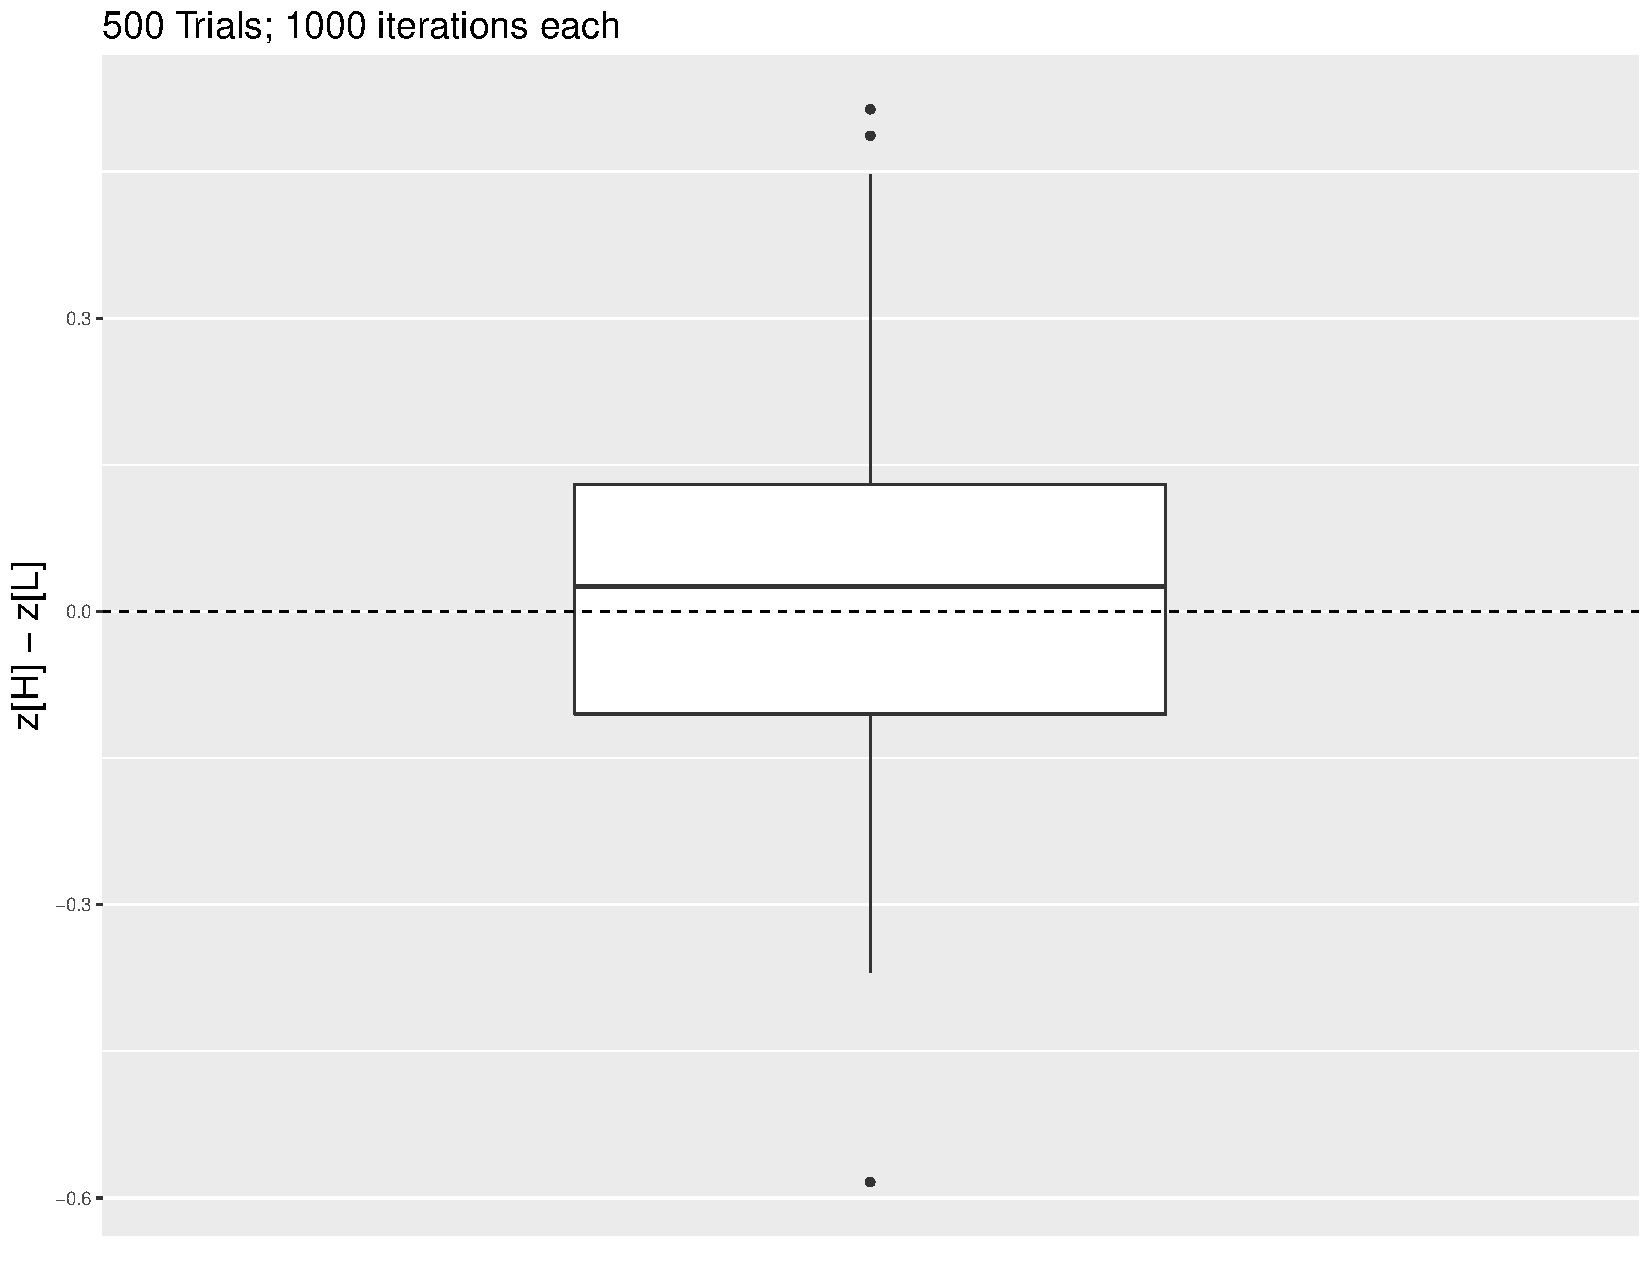
\includegraphics[width=\linewidth]{figures/FrequencyEffect.pdf}
        \caption{\label{fig:HvL}4:1 Token ratio}
    \end{subfigure}\hfill
    \begin{subfigure}[t]{.45\textwidth}
        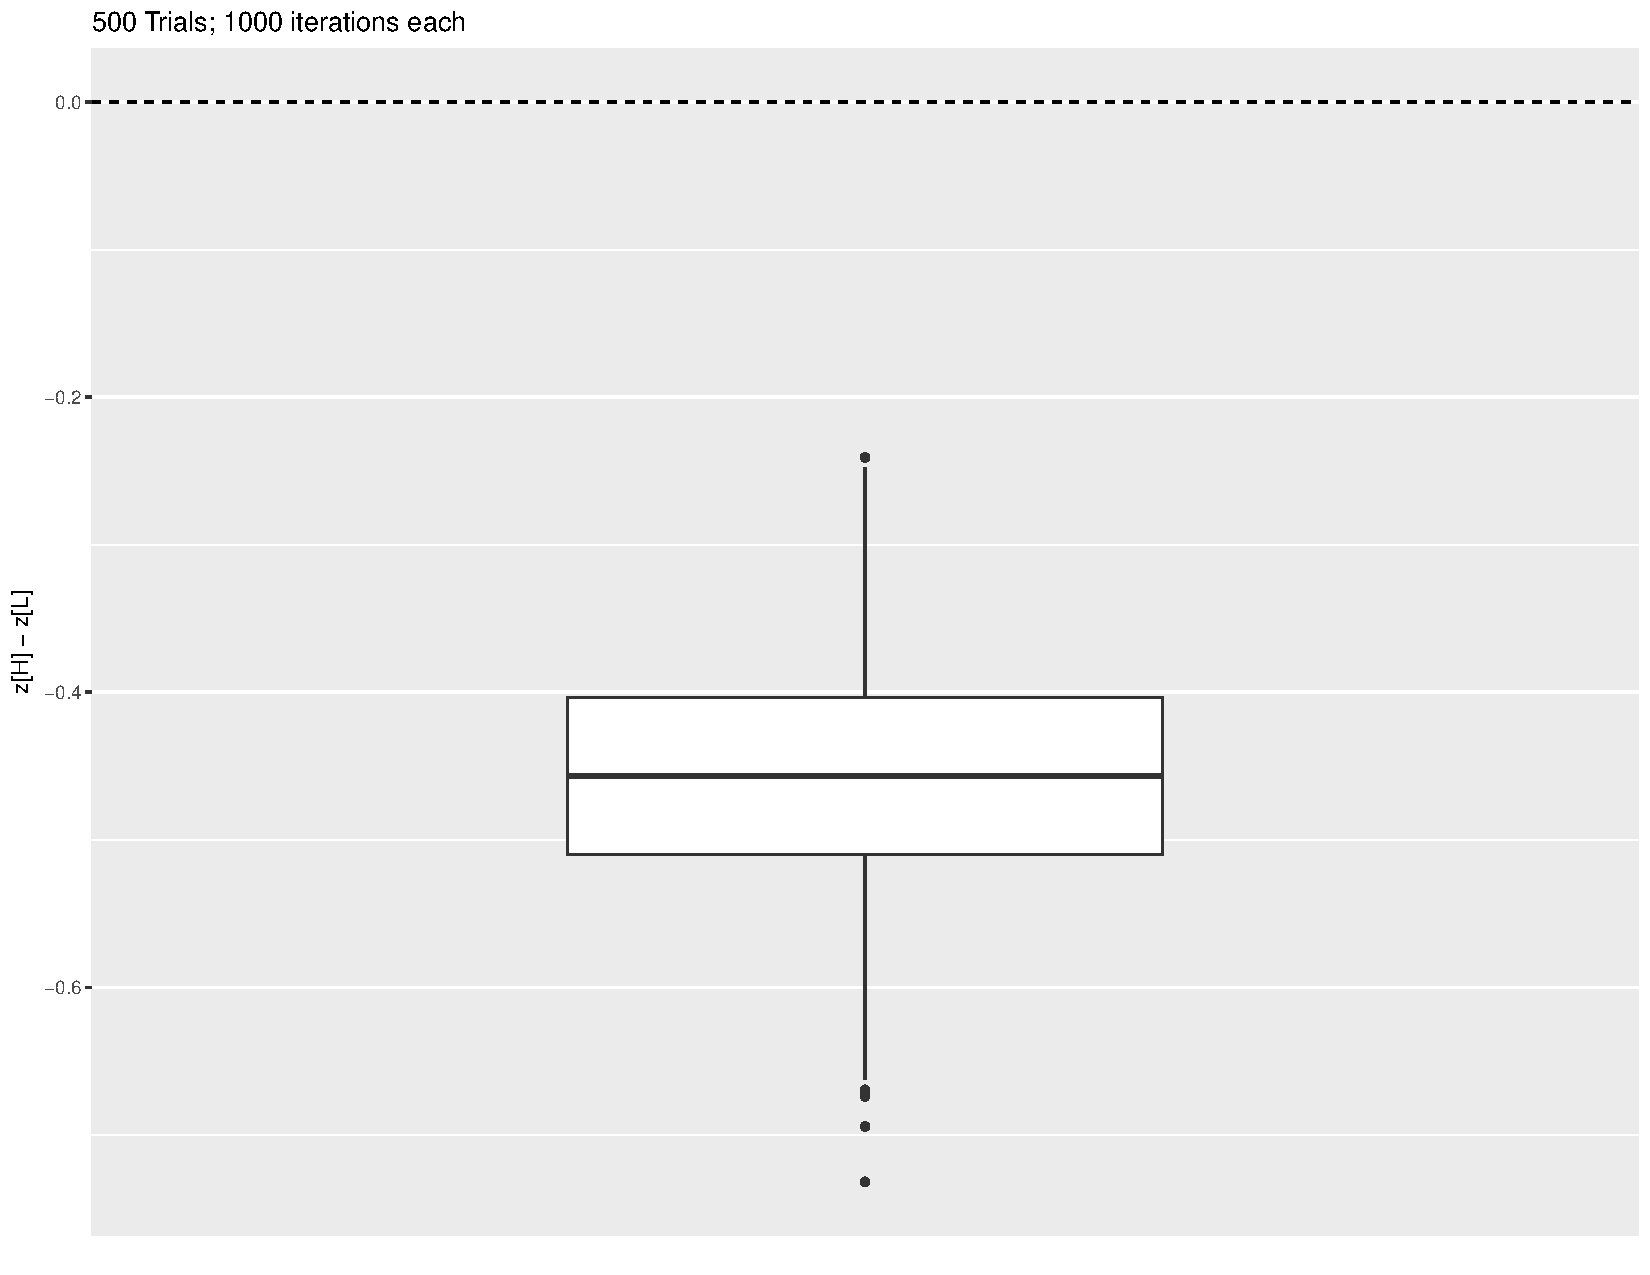
\includegraphics[width=\linewidth]{figures/FrequencyEffectEqNums.pdf}
        \caption{\label{fig:Freq.EqualTokens}1:1 Token Ratio}
    \end{subfigure}
% % \centering{}\subfloat[\label{fig:HvL}4:1 Token ratio]{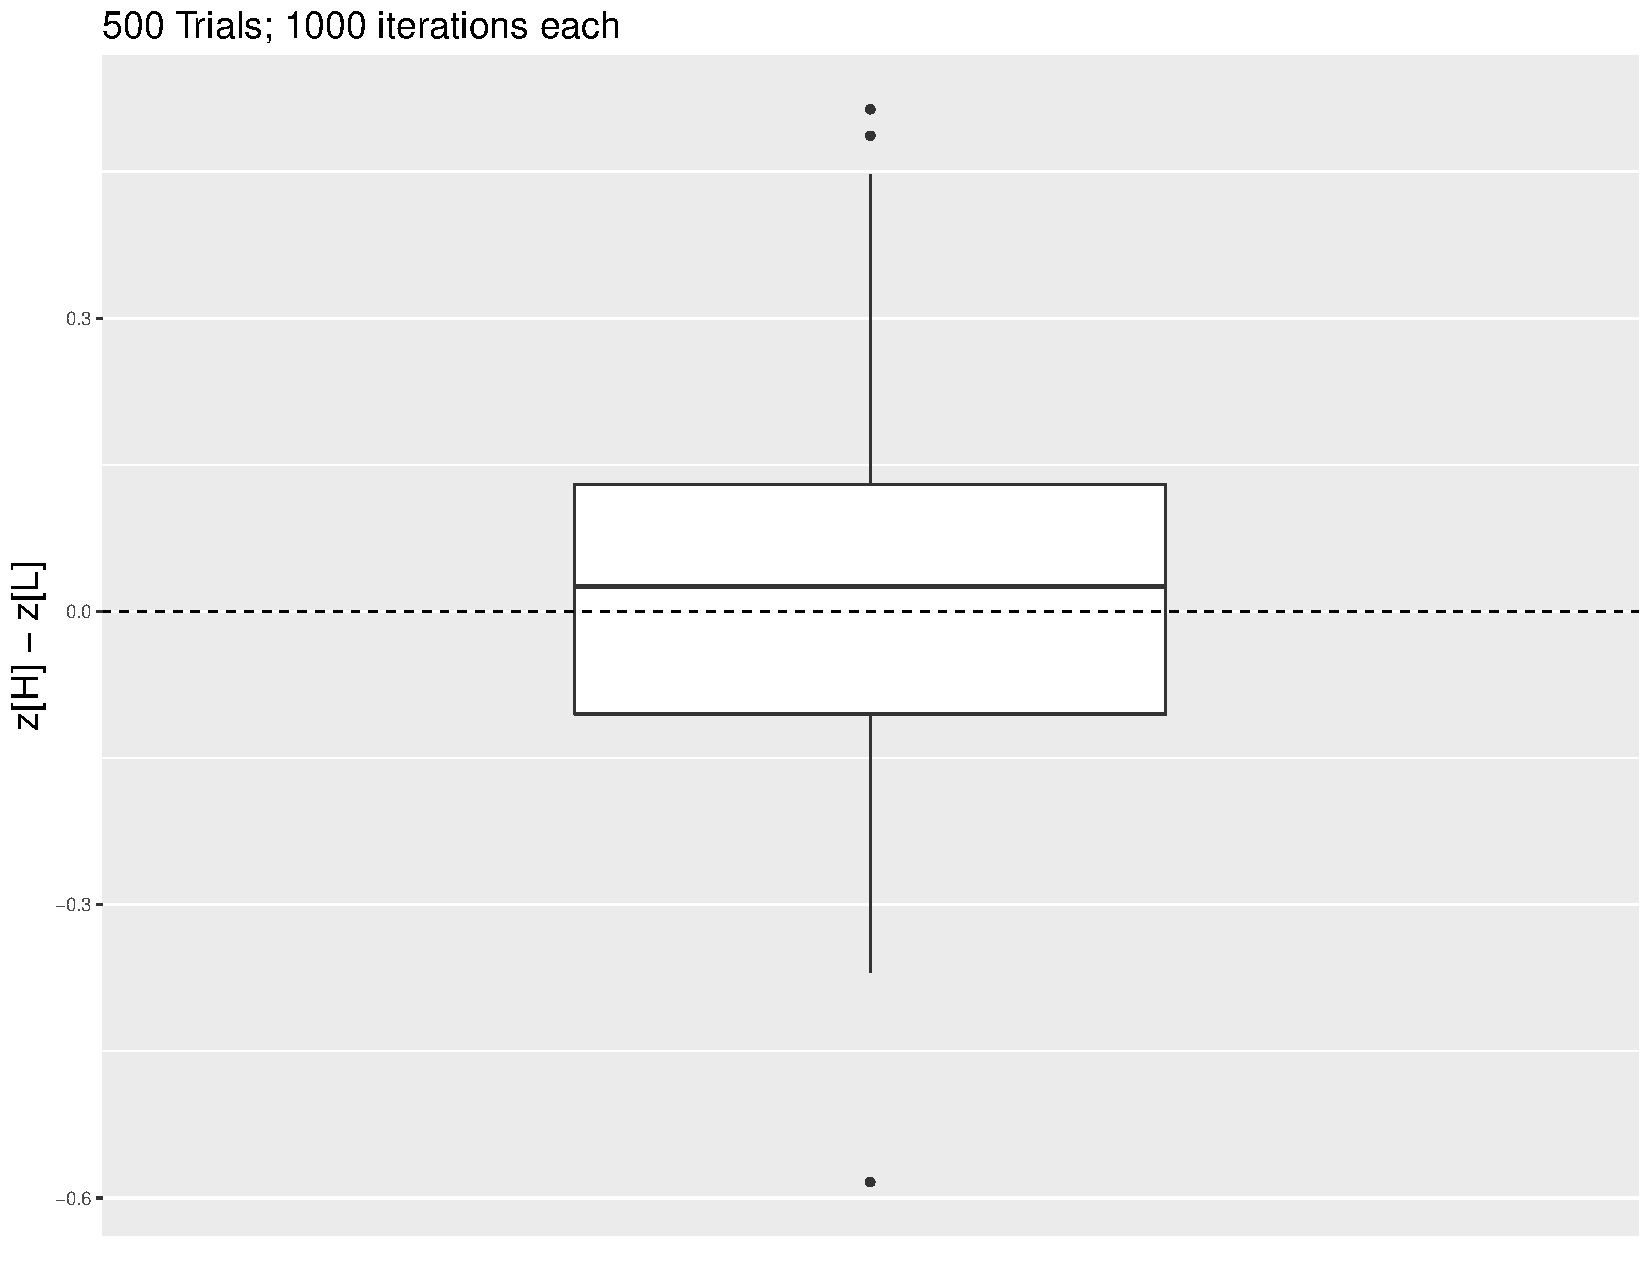
\includegraphics[width=0.3\textwidth]{figures/FrequencyEffect.pdf}}\hfill{}\subfloat[\label{fig:Freq.EqualTokens}1:1 Token Ratio]{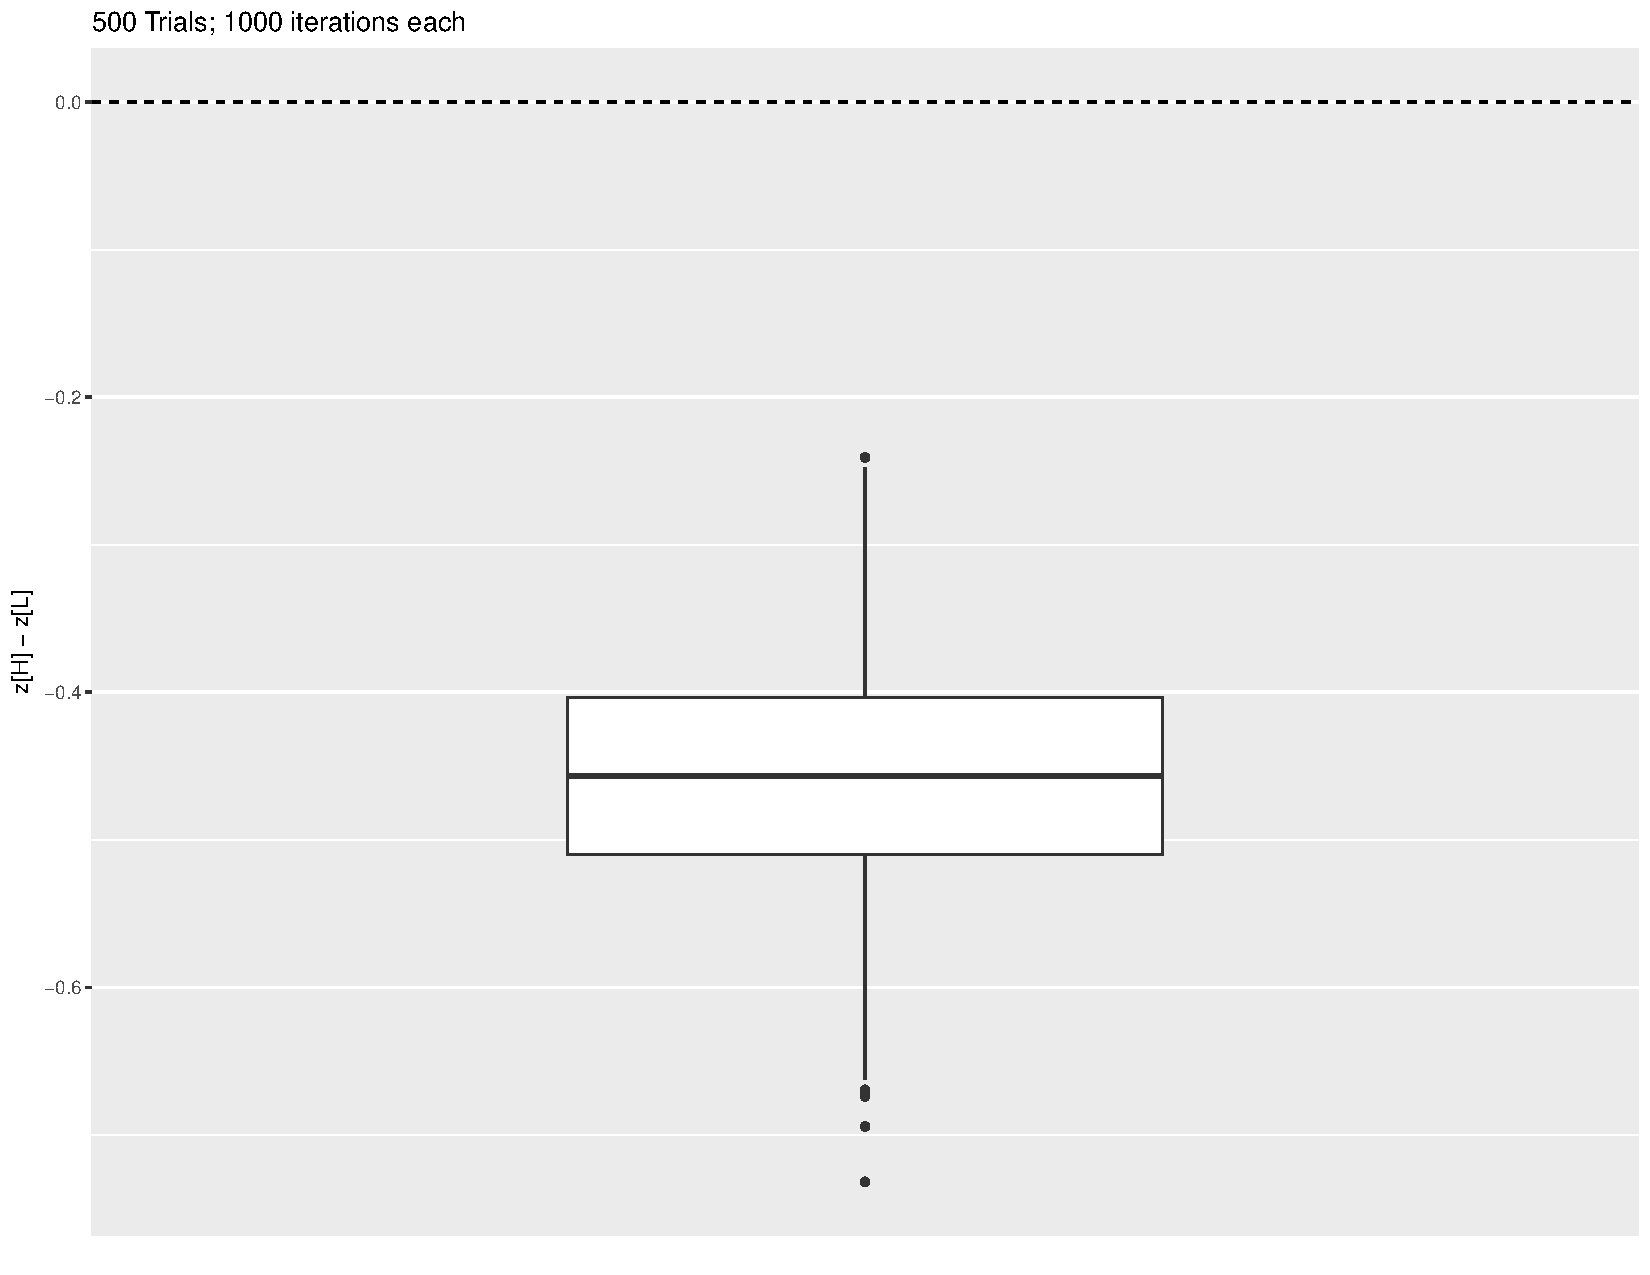
\includegraphics[width=0.3\textwidth]{figures/FrequencyEffectEqNums.pdf}}
\caption{Simulation of Iterative Biasing for H(igh) frequency category versus
L(ow) frequency category}
\end{figure}

The difference in the number of tokens in each category also results
in a difference in variance across the different trials. The variance
is larger for the lower-\isi{frequency} category due to undersampling; because
fewer tokens are produced from the low-\isi{frequency} category in a given
trial, and the tokens are selected randomly, the likelihood that the
sample will be significantly different from trial to trial is greater
(\citealt{Soskuthy} finds a similar effect using a parameterized \isi{exemplar}
model). Variance compounds over iterations, such that the variance
between independent model runs after 10,000 iterations is greater
than after 5000 iterations. \figref{fig:Frequency Catch Up} illustrates
the across-trial variance for the two categories at successive intervals,
after 500, 1000, 1500, and 2000 iterations.

\begin{figure}[H]
\centering{}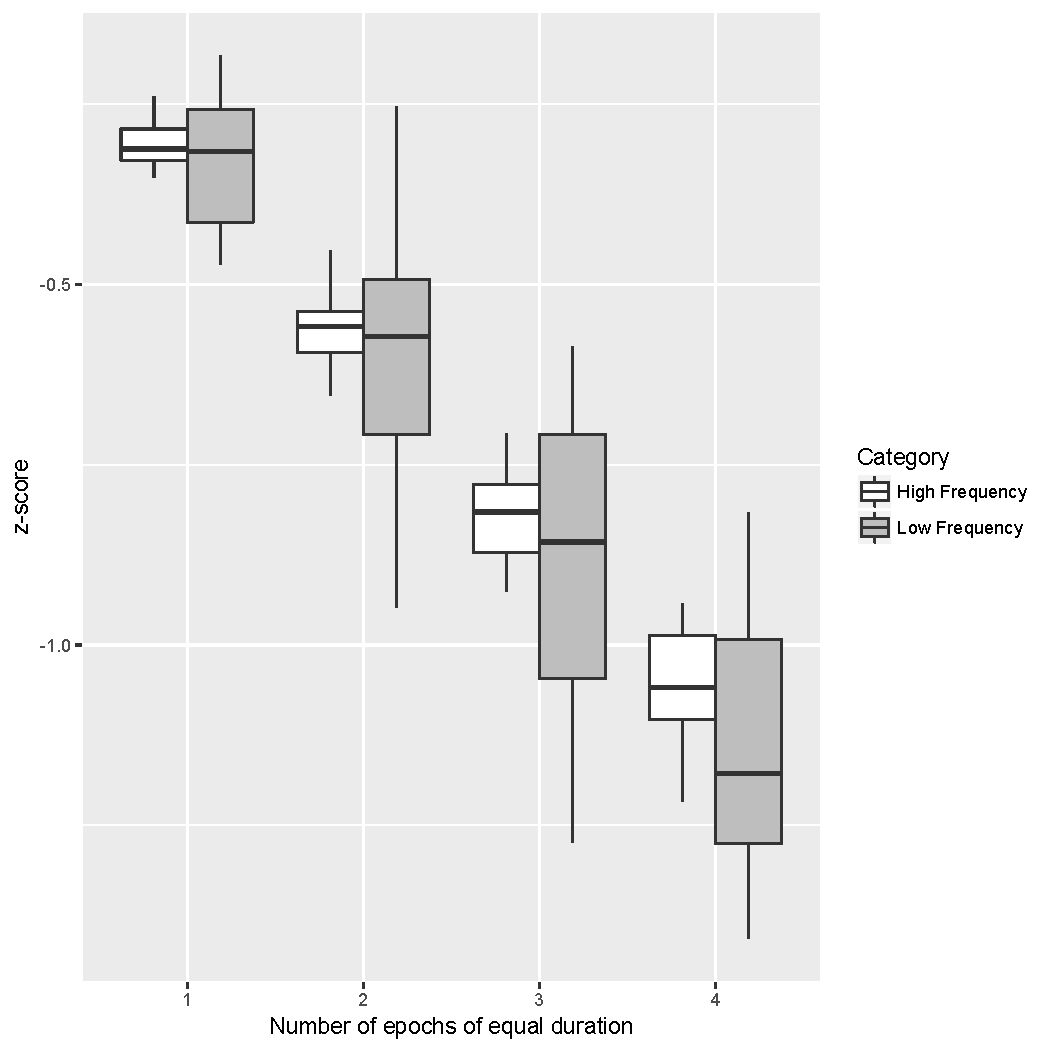
\includegraphics[width=.75\textwidth]{figures/FrequencyOverTime.pdf}\caption{\label{fig:Frequency Catch Up}Average z-scored value for High (white)
versus Low (gray) frequency categories at 4 equally spaced intervals
of model time, each 500 model iterations in duration (1 epoch). Each boxplot shows
the results of 10 independent trials at each of the successive epochs.}
\end{figure}

Different implementational choices and assumptions will produce somewhat
different results. If the two categories contain the same constant
number of tokens, but the high-\isi{frequency} category is still 4 times
more likely to be produced on any given iteration, then the high-\isi{frequency}
category will have a consistently lower value along \emph{x} than
the low-\isi{frequency} category. The results of the equal-tokens simulations are shown in \figref{fig:Freq.EqualTokens}.
This is because the \isi{inertia} from the larger number of few-times-biased
tokens is missing. These specific results also depend on the ratio
of frequencies of the two categories, as well as a number of other
parameter settings. Those dependencies will be discussed further in
Section \ref{subsec:Word-Frequency}, when this model is linked to
the linguistic phenomenon of frequency-based word reduction. For now,
we turn to the behavior of the model in the limit.

The means of both categories steadily decrease as a function of the
number of model iterations. Although the amount of biasing becomes
steadily smaller as token values become smaller, biasing is unbounded.
That is, the model does not converge on a stable state. Convergence
can be imposed by specifying a minimum value on \emph{x} beyond which
tokens cannot be reduced. This results in a skewed distribution with
a narrow peak at the threshold value and a small rightward tail due
to the normally distributed error term. The thresholded model clearly
illustrates that all categories, whether high or low \isi{frequency}, will
eventually end up at exactly the same minimum value, collapsing any
difference between them. 

\subsection{\label{sec:Context-Dependent-Iterativity}Context-dependent iterativity}

In the previous model all tokens of each category were subjected to
the same \isi{production} \isi{bias} – the context in which the tokens were produced
did not matter. The next two models are context-dependent models.
In these models the \isi{production} \isi{bias} only applies to a subset of tokens,
those produced in the biasing context. As before, \isi{production} tokens
are chosen at random; they are then produced in either a biasing or
non-biasing context, with a certain fixed probability. Regardless
of \isi{production} context, however, all tokens are added back to the same
originating category.

\subsubsection{\label{subsec:Phrase-Final Lengthening}Model 2: Gradient context-dependent bias}

Model 2 implements a gradient \isi{production} \isi{bias}, similar to the one
used in Model 1, but with an increasing, rather than decreasing, function
of $x$. On each iteration, the randomly selected token has probability
\emph{p} (< 0.5) of increasing by a fixed percentage ($\alpha$) of
its current value. As before, the category is initialized by sampling
from a normal distribution, and all tokens begin with non-biased values.
Because there is only one cloud in \isi{perception}, the only time a difference
between biased and non-biased tokens can be observed is at the moment
of \isi{production}. Therefore, model outputs will be given in terms of
an observed random sample of fixed size at some cycle, \emph{n}, of
the model.

The \isi{iterativity} of the perception-\isi{production} loop allows for tokens
to be biased multiple times, but also for tokens to remain persistently
non-biased, the more so the larger the category is in terms of stored
exemplars, and the smaller the value of \emph{p}. To understand model
behavior it is useful to think of each iteration as involving four
possible outcomes. In the first, a relatively low-valued token (the
outcome of a series of productions occurring more often in non-biasing
contexts) is chosen for \isi{production}, but this time in a biasing context,
thus increasing its value along \emph{x}. The second possibility is
that the same token is chosen for \isi{production} in a non-biasing context,
such that its value remains more or less unchanged (still relatively
low). The third and fourth possibilities involve selecting a relatively
high-valued token (the outcome of a series of productions occurring
more often in the biasing context) and either producing it in a non-biasing
context (no increase along \emph{x}), or a biasing context (additional
increase along \emph{x}). 

The last type of outcome ensures that a subset of tokens will continue
to increase without bound. Despite the fact that the second type of
outcome ensures the persistence of low-valued tokens, the category
as a whole will move unboundedly rightward along \emph{x}. This is
due to the combined effect of \isi{memory decay} and \isi{entrenchment}. For $p<0.5$,
the overall mean of the distribution will always be closer to the
lower-valued side of the distribution, and will initially act to oppose
the increase due to \isi{production} \isi{bias}. However, as higher-valued tokens
are added to the category, they seed even higher-valued daughter tokens,
generating an exponentially increasing subset of tokens. This is the
relationship expressed in Eq. (\ref{eq:linear bias}), reformulated
here, for a positive \isi{bias}, as $x_{o(+n)}=x_{o}(1+\alpha)$. As this
subset of tokens moves right, it will drag the rest of the distribution
with it. \figref{fig:End context mismatch} illustrates this effect
via comparison of the observed distribution after a model run of 1,000
iterations, versus 5,000 iterations.

\begin{figure}[H]

\begin{subfigure}[t]{.45\textwidth}
        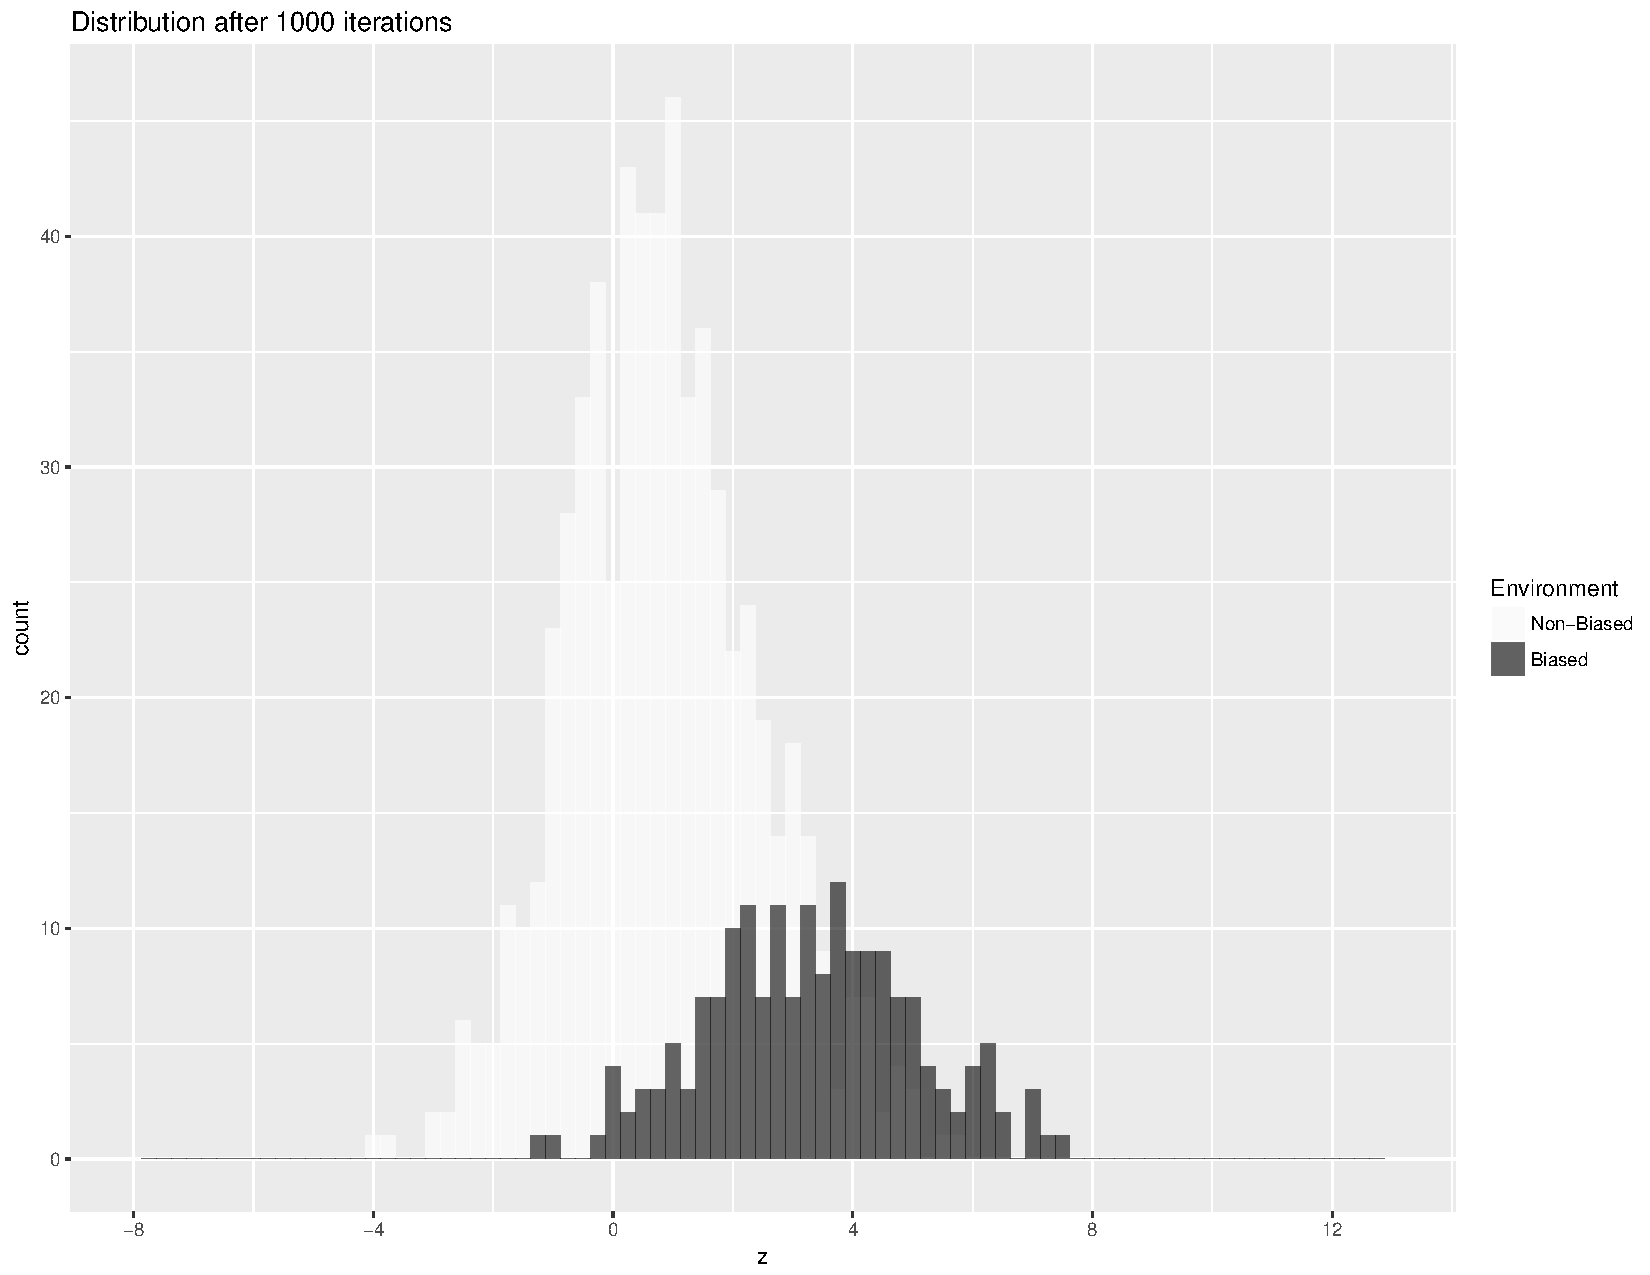
\includegraphics[width=\linewidth]{figures/1000iter.pdf}
        \caption{1000 iterations}
    \end{subfigure}\hfill
    \begin{subfigure}[t]{.45\textwidth}
        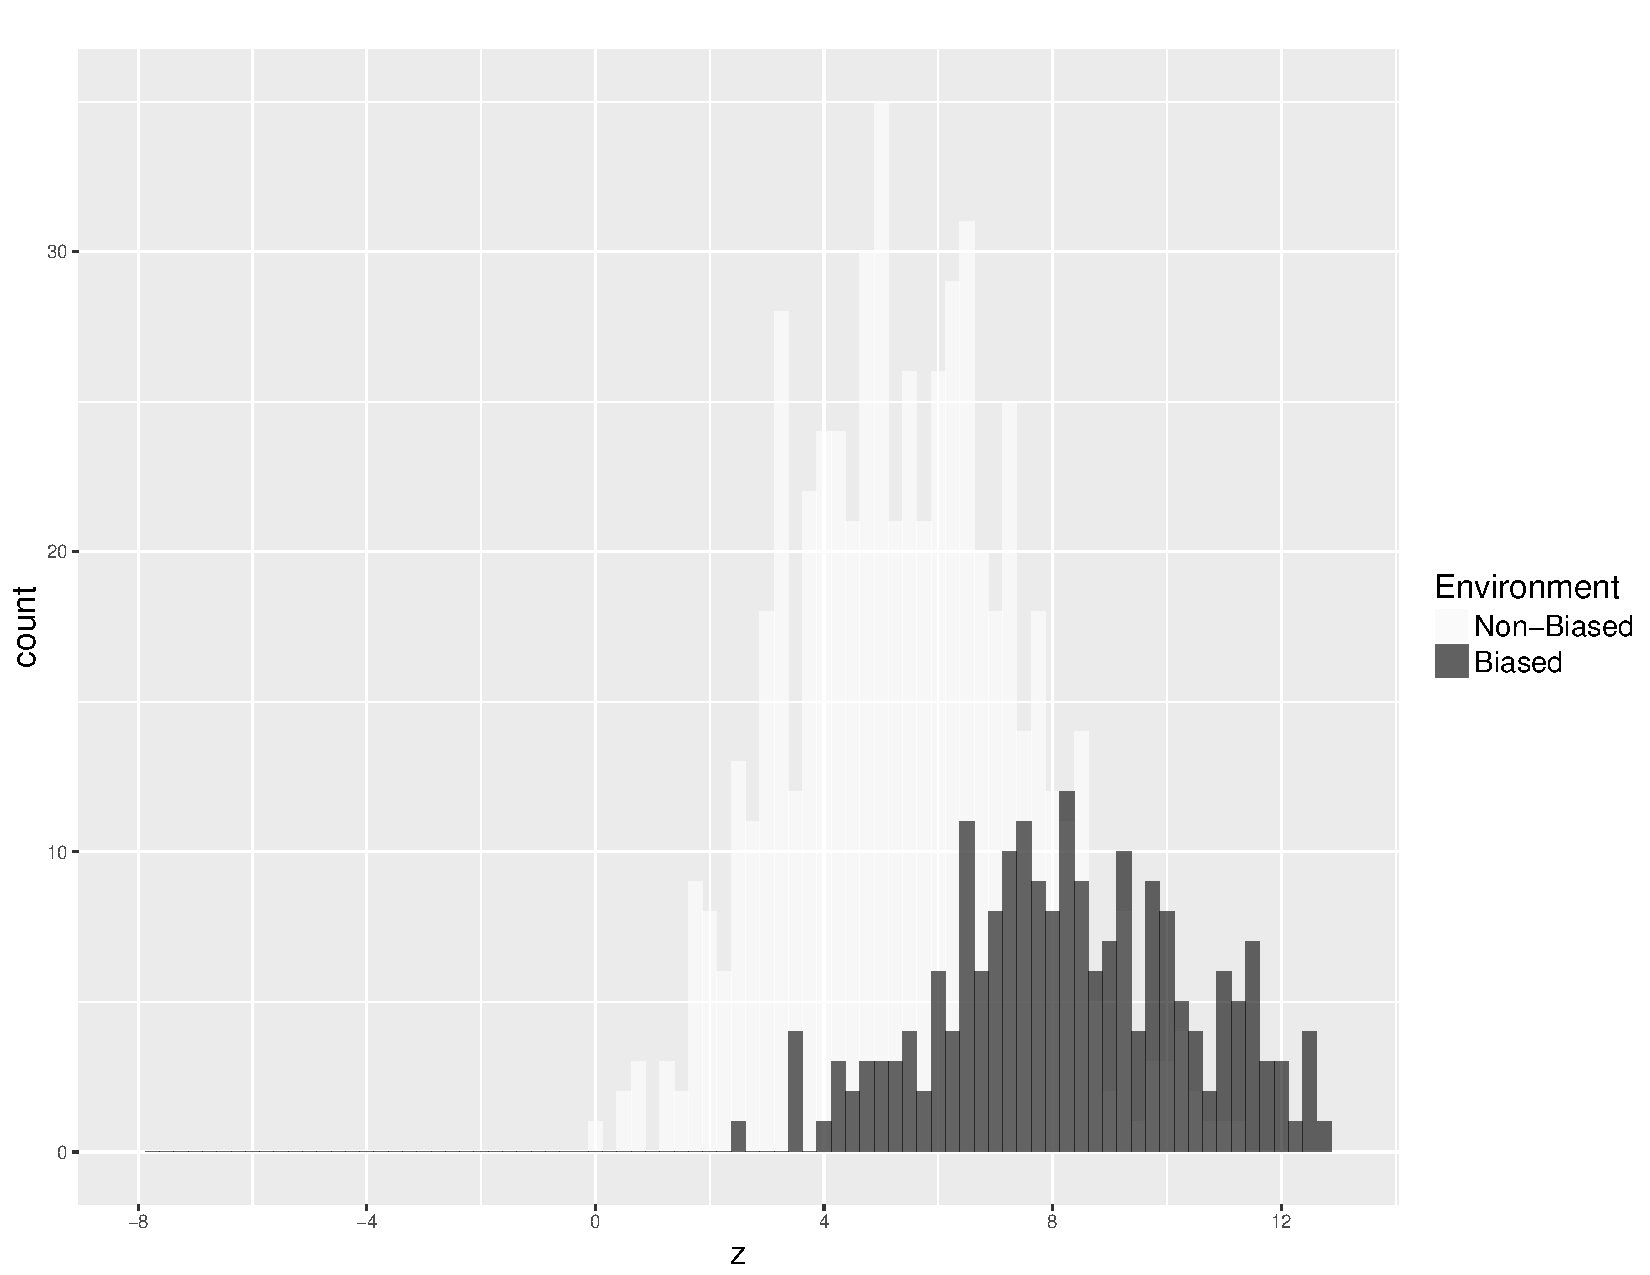
\includegraphics[width=\linewidth]{figures/5000iter.pdf}
        \caption{5000 iterations}
    \end{subfigure}
    
% % \subfloat[1000 iterations]{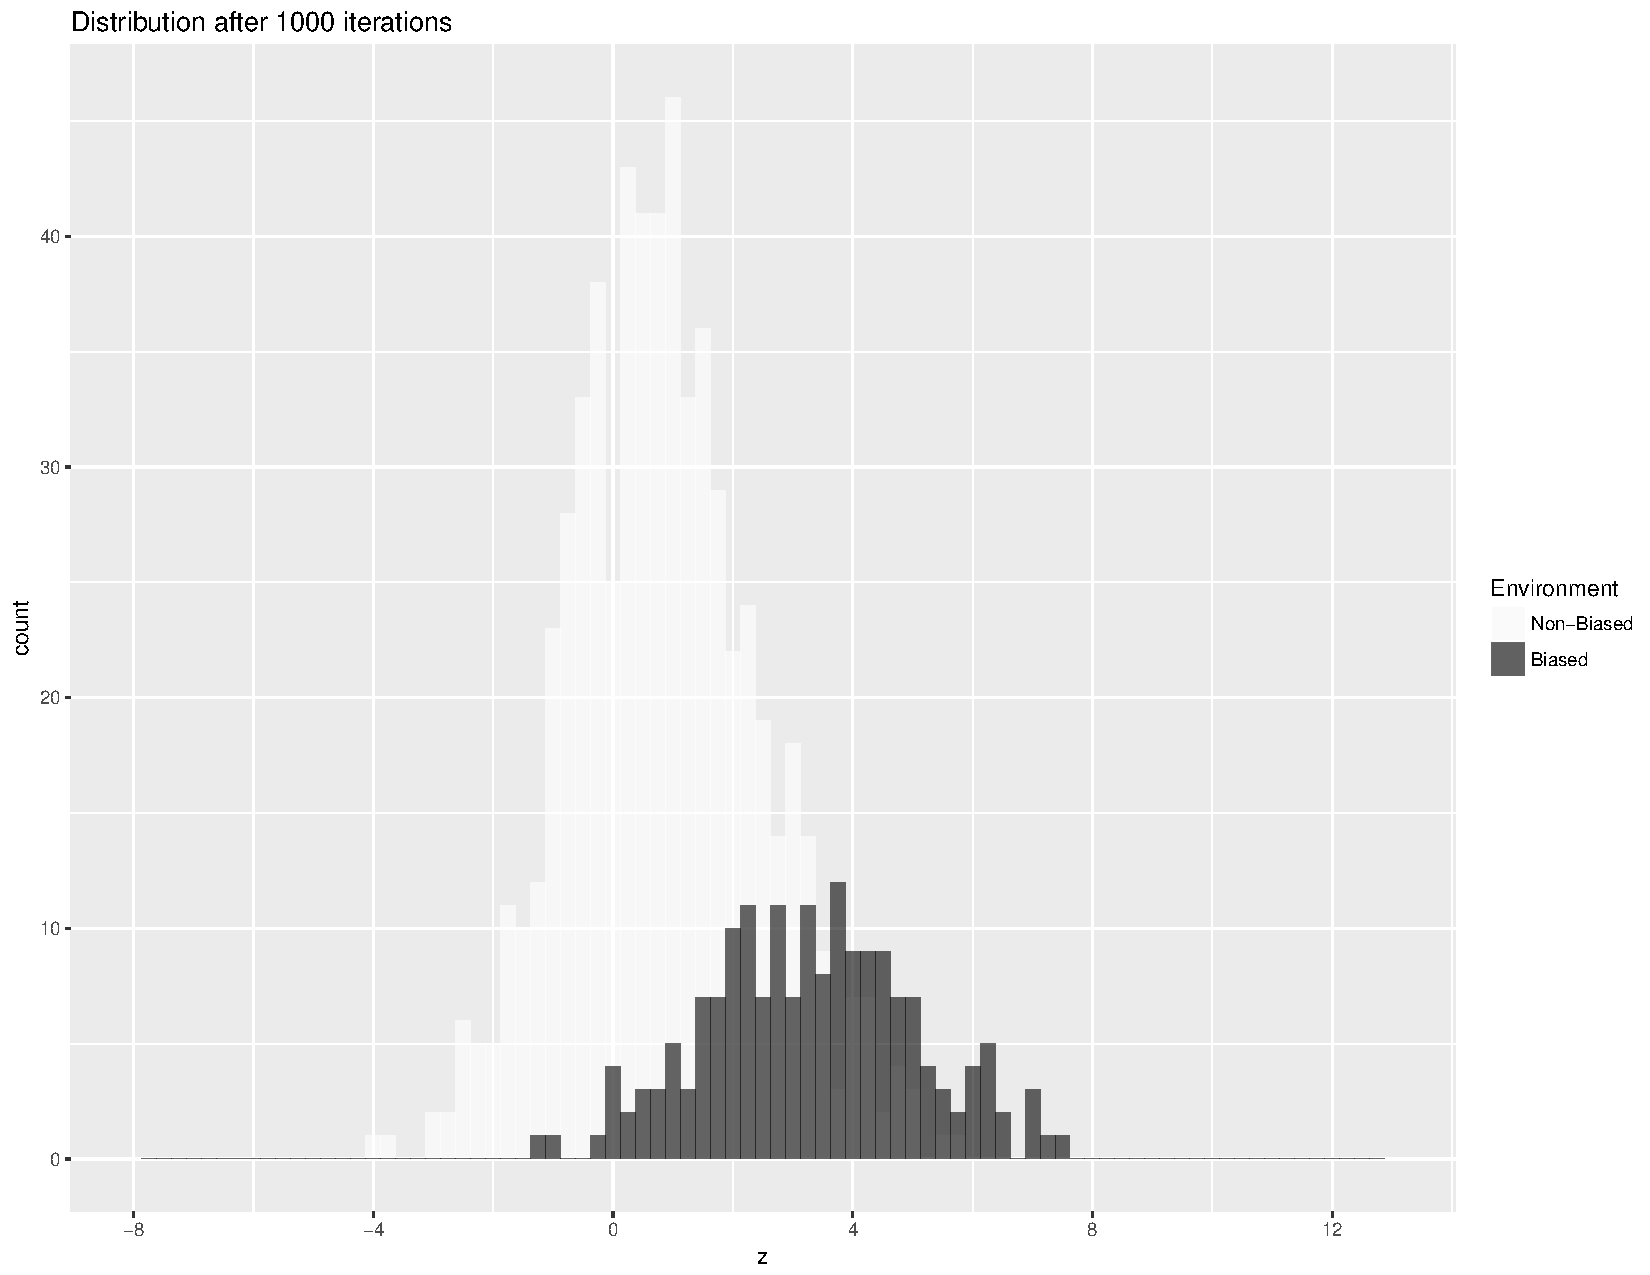
\includegraphics[width=0.3\textwidth]{figures/1000iter.pdf}}\hfill{}\subfloat[5000 iterations]{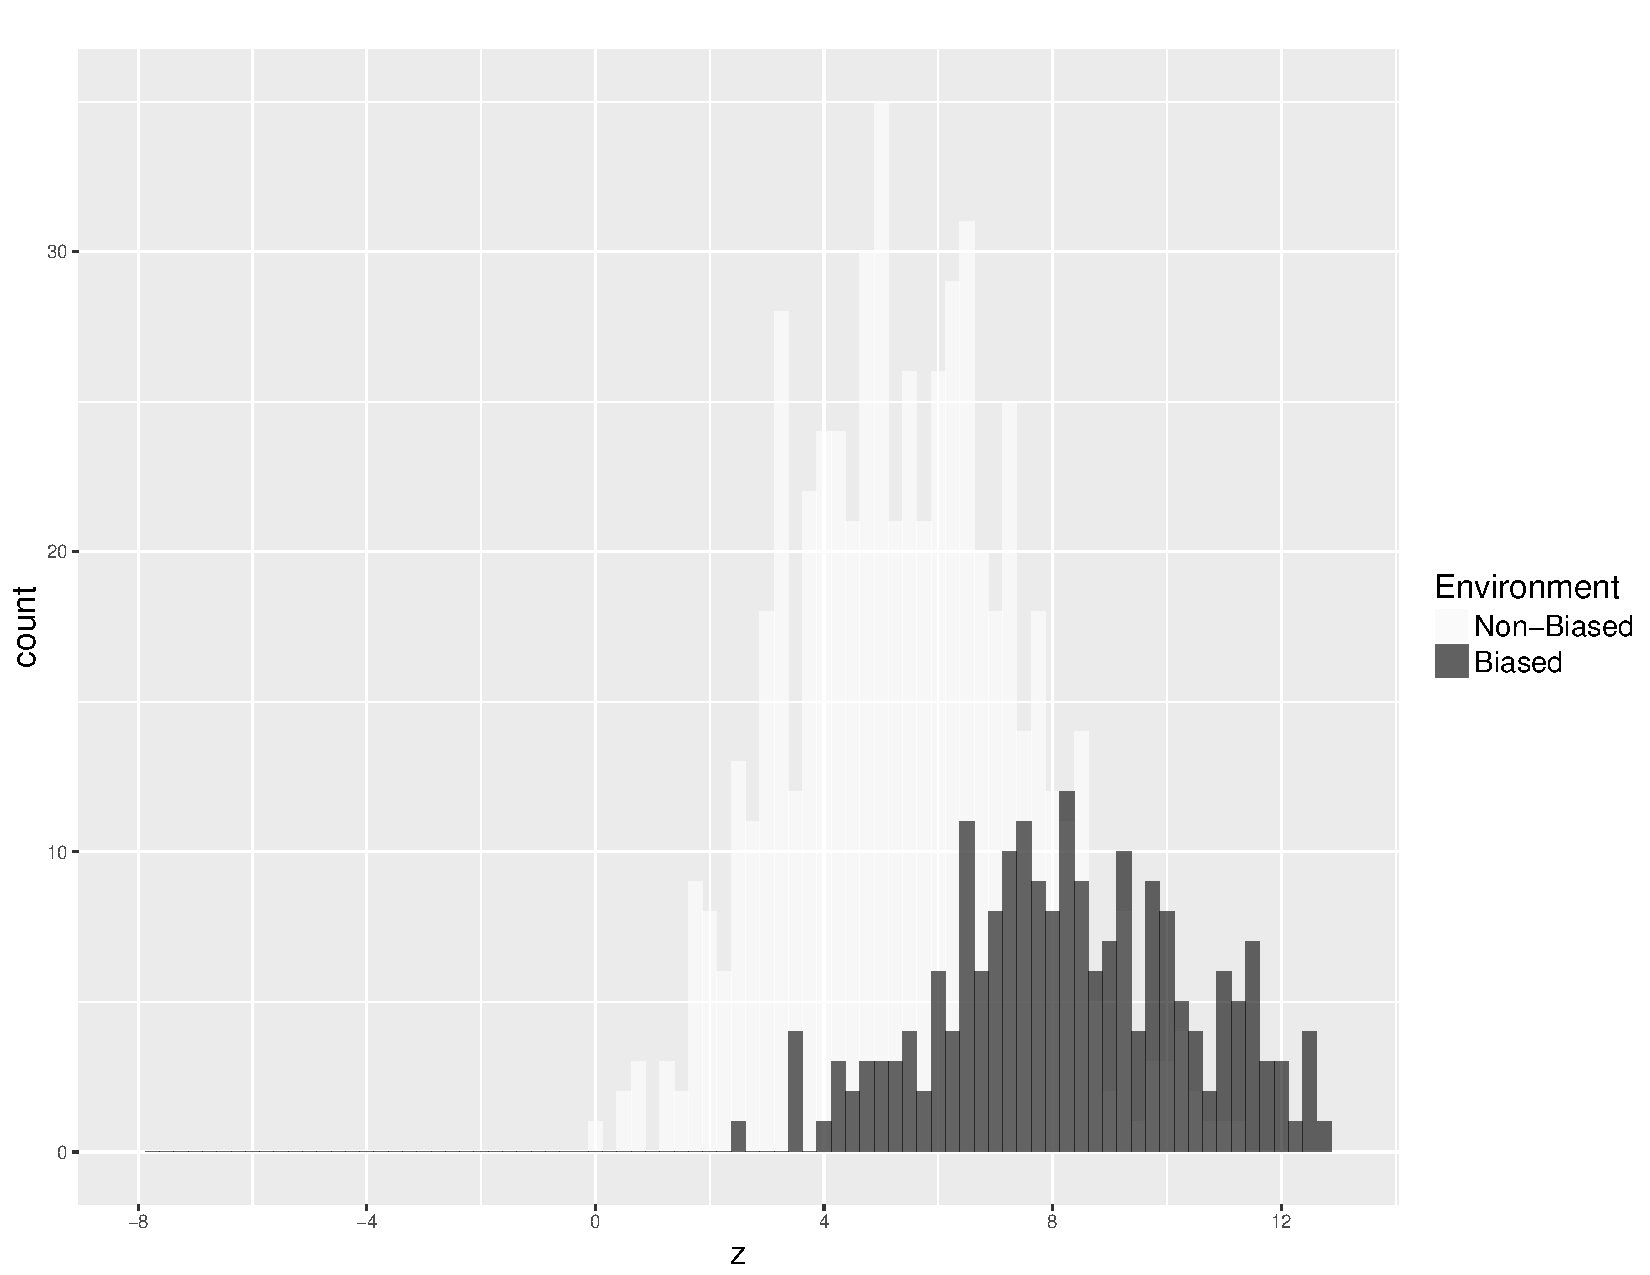
\includegraphics[width=0.3\textwidth]{figures/5000iter.pdf}}

\caption{\label{fig:End context mismatch}Observed distribution (800 tokens).
White: productions in non-biasing context. Black: productions in biasing
context.}
\end{figure}

As expected, the same unboundedness problem arises as was seen in
Model 1. With the addition of a threshold (ceiling or floor value
along \emph{x}) the sub-distributions merge, neutralizing the difference
between biased and non-biased contexts.\footnote{\citet{DBLP:journals/corr/Tupper14a} attributes a merged outcome
such as this to perfect categorization accuracy, i.e., failure to
discard ambiguous tokens. } It will also be shown that keeping all tokens in the same category,
regardless of history, results in another type of problem – what I
will call \isi{context mismatch}. Context mismatch will be discussed when
this model is linked to the linguistic phenomenon of vowel \isi{lengthening}
in Section \ref{subsec:Model-2:-Lengthening}.

\subsubsection{\label{subsec:Model-3:-Categorical}Model 3: Categorical context-dependent bias}

Model 3 implements a binary \isi{production} \isi{bias}, albeit with an error
term that maintains a small amount of variance. All tokens produced
in the biasing context are initialized with a mean at the {[}+{]} value
on dimension \emph{x}, while all tokens produced in the non-biasing
context are initialized at the {[}\textminus{]} value. See \figref{fig:binary-Starting-Distribution}.
As before, all tokens belong to the same category; the different colors
are for illustrative purposes only, allowing us to track the \isi{production}
context during the observation cycle. Because the \isi{bias} is uni-directional,
and biasing is categorical, all tokens quickly shift to the biased
{[}+{]} value. Once a token has a value of /+/ it cannot be biased
further, nor can it be ``un-biased''. This is shown in \figref{fig:binary-1000iter},
where we can see that previously biased tokens remain at {[}+{]} even
if they are subsequently produced in a non-biasing context (white
bars at {[}+{]} location). This model is, in fact, bounded, because
there is no \isi{iterativity} for the binary feature. However, like the
previous two models, it results in neutralization of the difference
between the different contexts. Binary-valued features that distinguish
between contrastive sound units within a language are widely used
in \isi{phonological} theory. This connection will be discussed when the
model is linked to the linguistic phenomenon of \isi{vowel nasalization}
in \sectref{subsec:Model-3:-Nasalization}.

\begin{figure}[H]

\begin{subfigure}[t]{.45\textwidth}
        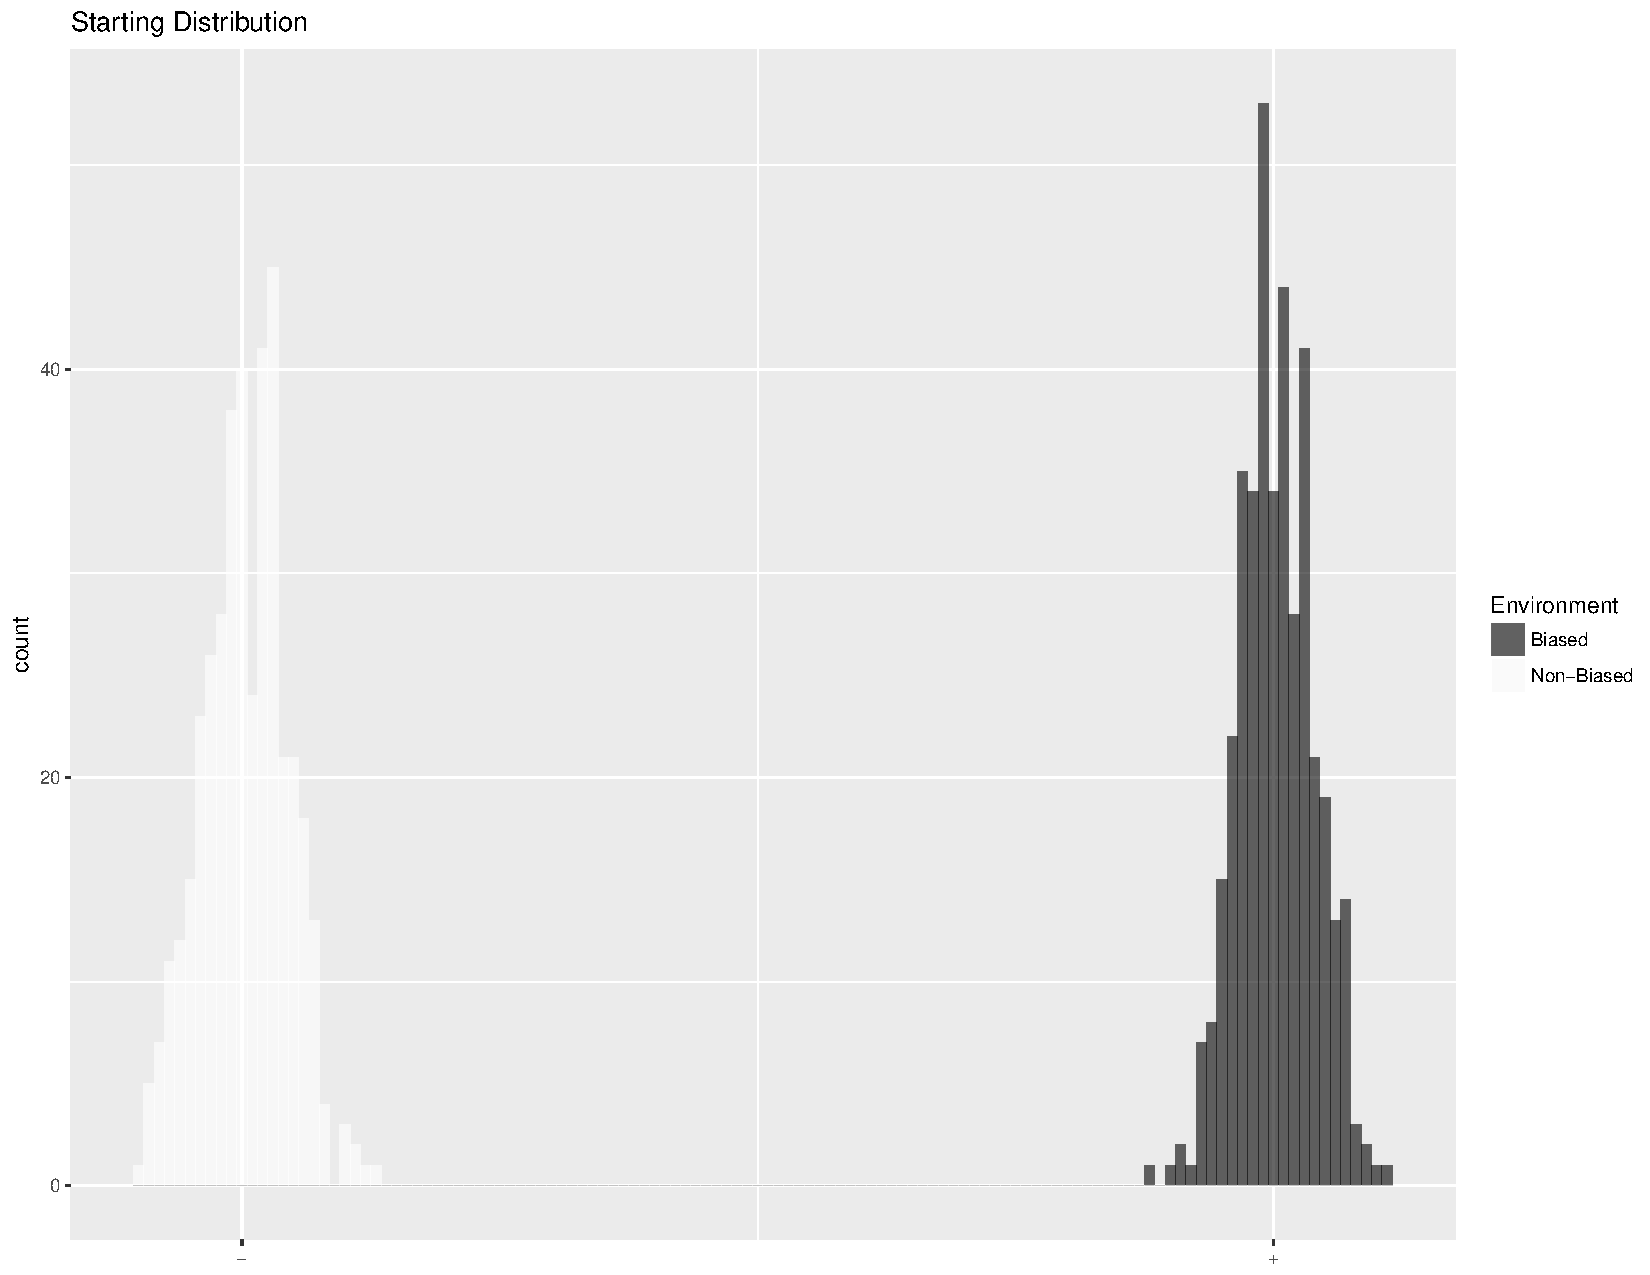
\includegraphics[width=\linewidth]{figures/NasalizationStart.pdf}
        \caption{\label{fig:binary-Starting-Distribution}Starting Distribution}
    \end{subfigure}\hfill
    \begin{subfigure}[t]{.45\textwidth}
        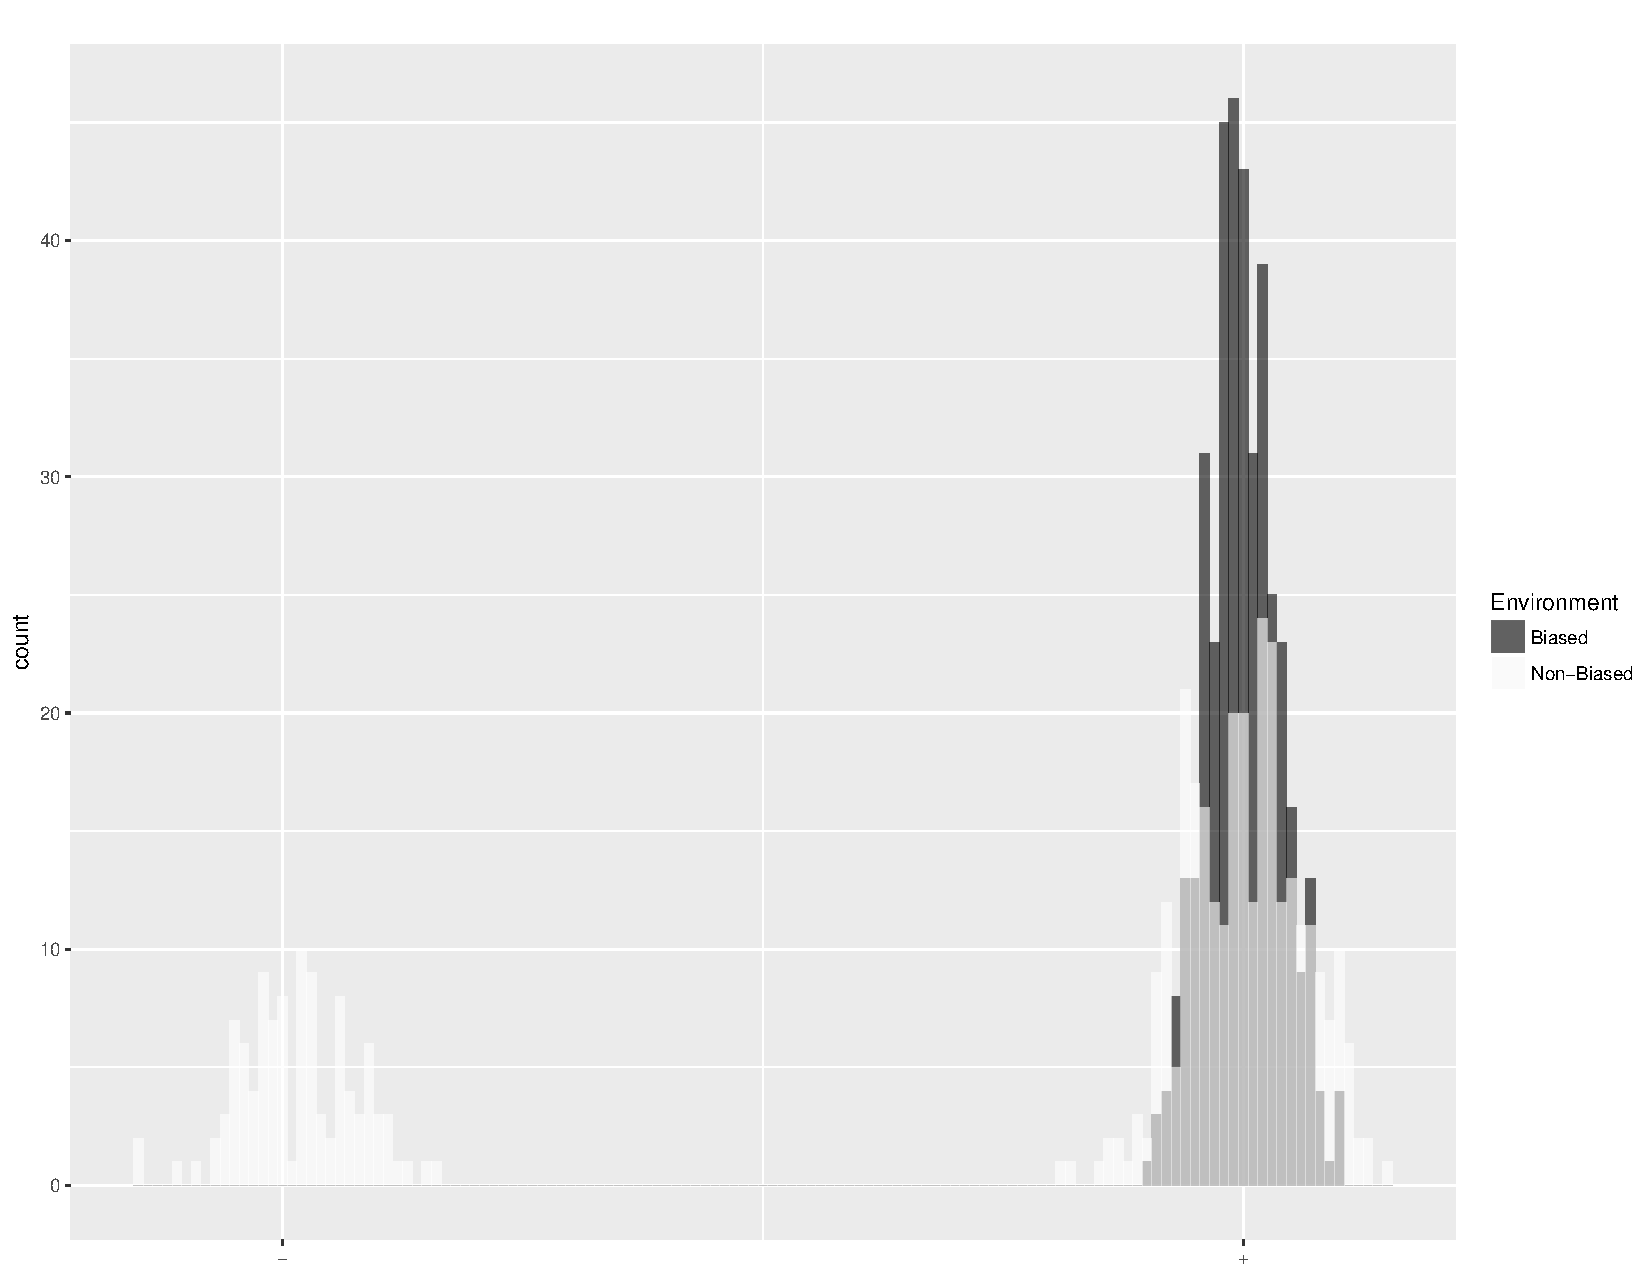
\includegraphics[width=\linewidth]{figures/Nasalization1000iter.pdf}
        \caption{\label{fig:binary-1000iter}1000 iterations}
    \end{subfigure}
% 
% \subfloat[\label{fig:binary-Starting-Distribution}Starting Distribution]{
% 
% 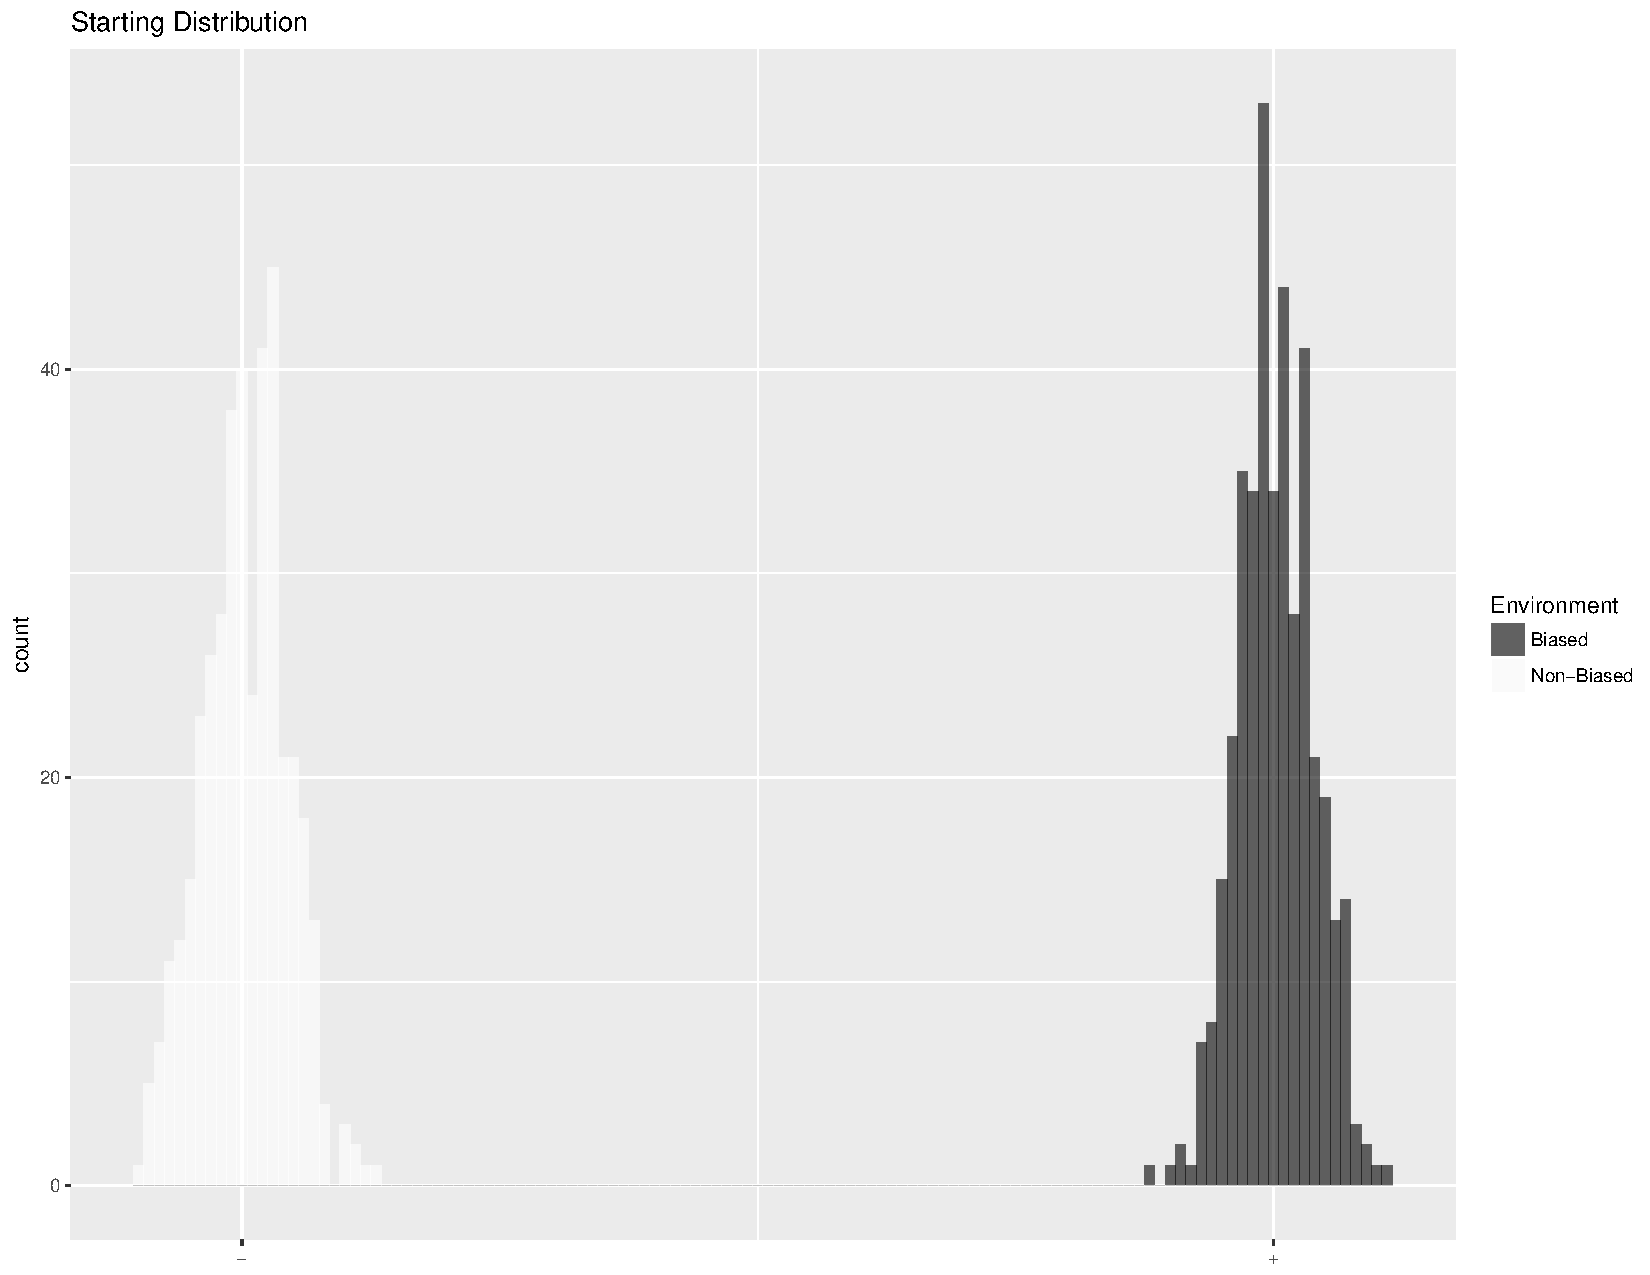
\includegraphics[width=0.3\textwidth]{figures/NasalizationStart.pdf}}\hfill{}\subfloat[\label{fig:binary-1000iter}1000 iterations]{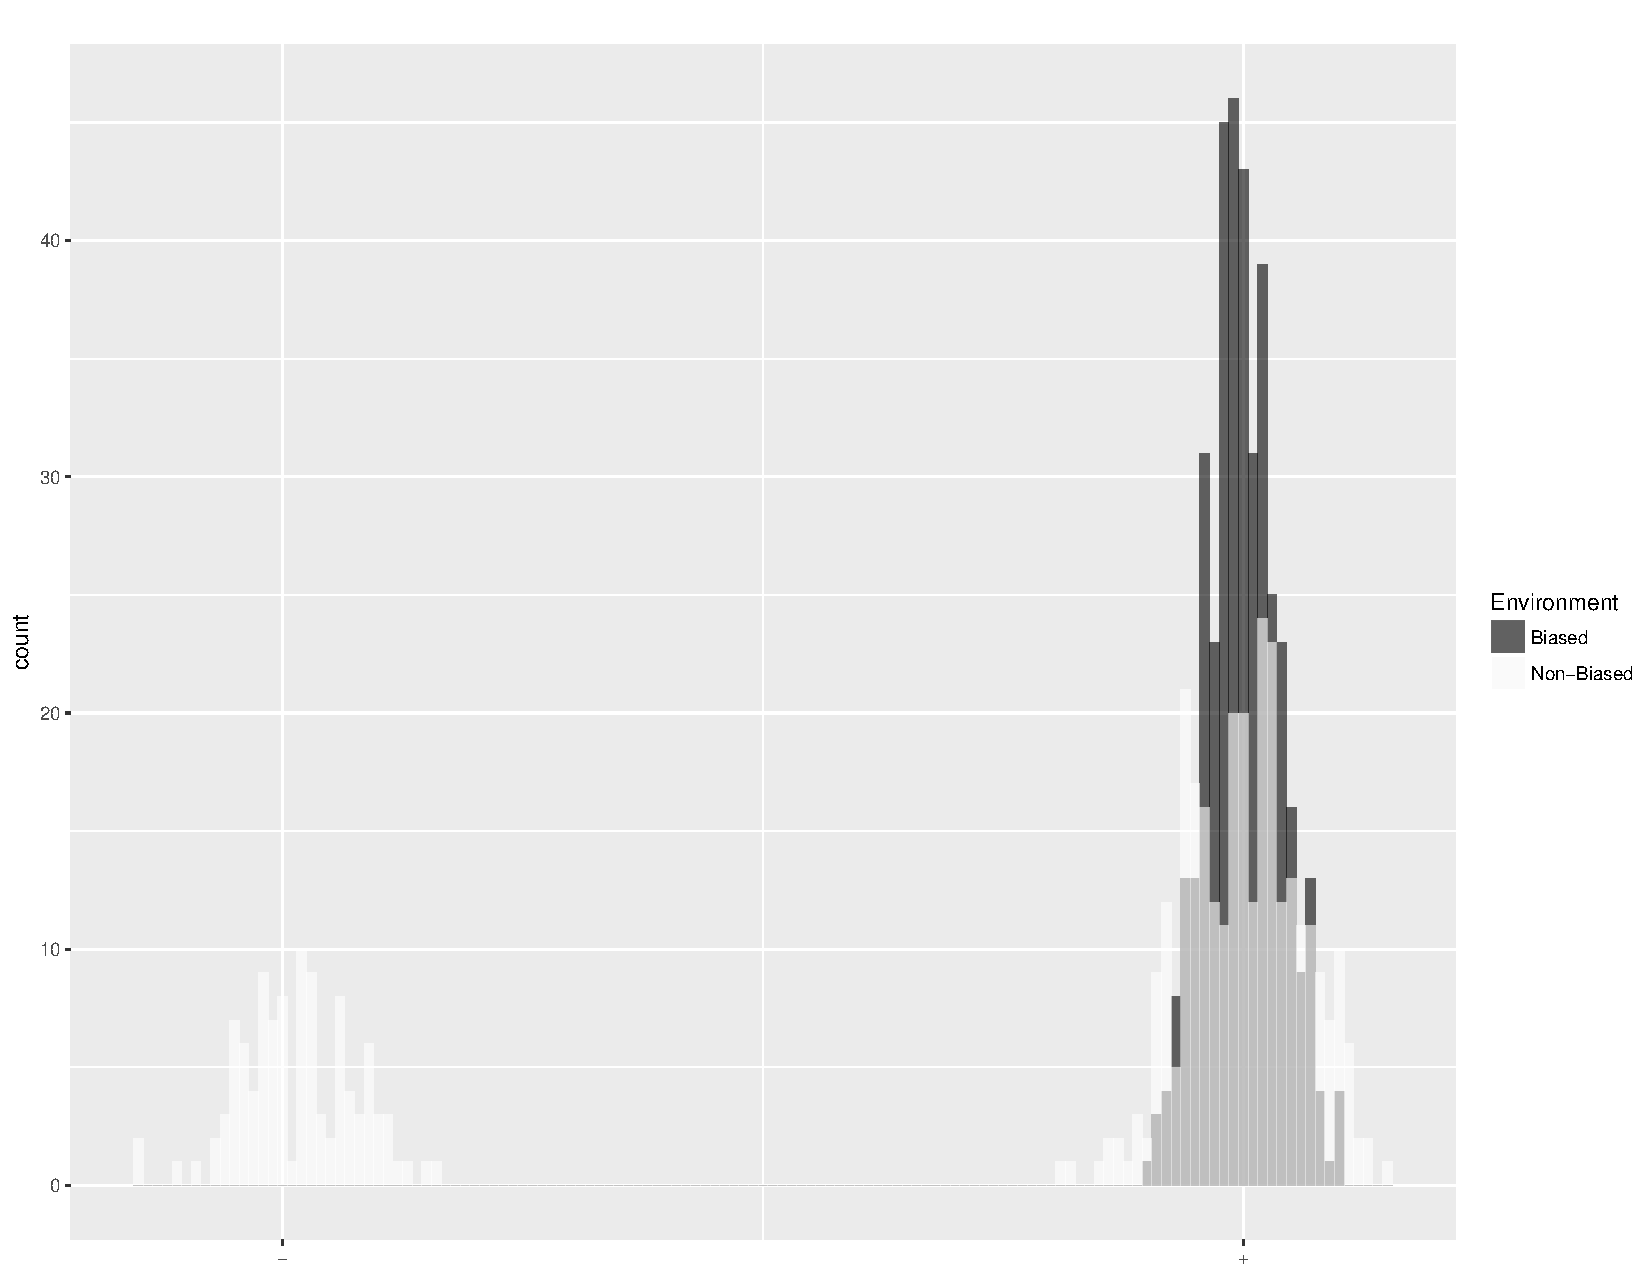
\includegraphics[width=0.3\textwidth]{figures/Nasalization1000iter.pdf}}

\caption{\label{fig:Context Mismatch Features}Quasi-binary feature. Two variants
with equal contextual frequency.}
\end{figure}
